\documentclass[a4paper, 12pt]{report}

\usepackage{graphicx}
\usepackage{setspace}
\usepackage{fontspec} 
\usepackage{tocloft}
\cftsetindents{table}{0em}{5em}
\renewcommand\cfttabpresnum{Table }
\usepackage{enumitem}
\usepackage[natbibapa]{apacite}
\usepackage{caption}
\usepackage{url}
\usepackage{minted}
\usepackage{mdframed}
\usepackage{eso-pic}
\usepackage{tikz}
\usepackage{ragged2e}
\usepackage{multirow}      % Multi-row cells
\usepackage{array}        % Enhanced column controls
\usepackage{booktabs}     % Better horizontal lines
\usepackage{siunitx}      % Scientific units
\usepackage{makecell}    % For controlled line breaks in cells
\usepackage{tabularx} 
\usepackage{pgfgantt}
\usepackage[table]{xcolor}
\usepackage{amsmath} 
\usepackage[margin=2.5cm, top=2cm, bottom=2.5cm]{geometry}
\usepackage{chngcntr}
\usepackage{polyglossia}
\setdefaultlanguage{english}
\setmainfont{Times New Roman}
\setotherlanguage{khmer}
\newfontfamily\khmerfont{KhmerOSbattambang.ttf}[Path=C:/Windows/Fonts/]
\newfontfamily\khmerfontmoul{KhmerOSmuollight.ttf}[Path=C:/Windows/Fonts/]
\newfontfamily\khmerfontsr{KhmerOSsiemreap.ttf}[Path=C:/Windows/Fonts/]

\usepackage{hyperref}
\hypersetup{
    colorlinks=false,       % false: boxed links; true: colored links
    linkcolor=black,        % color of internal links
    citecolor=black,        % color of links to bibliography
    filecolor=black,        % color of file links
    urlcolor=black          % color of external links
}
\setlength{\parindent}{0pt}

\newcommand{\progressbar}[1]{%
  \cellcolor{blue!25}\makebox[0pt][l]{\cellcolor{blue!50}\hspace{#1\linewidth}}%
  \hspace{-\linewidth}#1%
}

\newcommand{\hs}{
    \hspace{1.5cm}
}
\counterwithin{section}{chapter}  % Makes sections reset with each chapter
\counterwithin{subsection}{section}

\newcommand{\mychapter}[2]{
  \chapter*{#1}
  \addcontentsline{toc}{chapter}{#2}
  \refstepcounter{chapter} % Automatically increment chapter
  \setcounter{section}{0} % Reset section counter
  \label{chap:\thechapter}
}

\newcommand\Watermark{%
  \AddToShipoutPicture*{%
    \put(0,0){%
      \parbox[b][\paperheight]{\paperwidth}{%
        \vfill
        \centering
        \begin{tikzpicture}[overlay, remember picture]
          \node[anchor=center, opacity=0.2] at (current page.center) {%
            
\includegraphics[width=15cm]{images/schools/watermark.png} % Path to your logo image
          };
        \end{tikzpicture}
        \vfill
      }
    }
  }
}
\usepackage[T1]{fontenc}

\XeTeXlinebreaklocale 'khm'
\XeTeXlinebreakskip = 0pt plus 0.5pt minus 0.25pt

\newcommand{\unnumberdSection}[1]{
    \section*{#1}\addcontentsline{toc}{chapter}{#1}
}

\newcommand{\fg}[3]{
    \begin{figure}[H]
        \centering
        \includegraphics[width=#1]{#3}
        \caption{#2}
        \label{fig:#3}
    \end{figure}
}

\setcounter{secnumdepth}{3} % <<-- Add this line

\begin{document}
 % ================================================================ Cover Pages
 \begin{mdframed}[linewidth=1.5pt, roundcorner=5pt]
% skipabove=\dimexpr\topskip+4cm\relax, % Space above (adjust for header)
%skipbelow=\dimexpr\baselineskip+1cm\relax] % Space below (adjust for footer)] % Adjust linewidth for the border thickness

% Khmer section with logo and text
\begin{center}
    \begin{minipage}[t]{0.2\linewidth}
        % Content for the first part (left logo)
        \begin{center}
            
\includegraphics[scale=.5]{images/schools/moey.png}
        \end{center}
    \end{minipage}%
    \hfill
    \begin{minipage}[t]{0.6\linewidth}
        % Content for the second part (middle text)
        \vspace{-3.2cm} % Adjust the space as needed
        \begin{center}
            \fontsize{18pt}{15pt} \textbf{\khmerfontmoul ក្រសួងអប់រំ យុវជន និងកីឡា}\\
            \vspace{0.5cm}
            \fontsize{17pt}{15pt} \textbf{\khmerfontmoul វិទ្យាស្ថានបច្ចេកវិទ្យាកម្ពុជា}
        \end{center}
    \end{minipage}%
    \hfill
    \begin{minipage}[t]{0.2\linewidth}
        % Content for the third part (right logo)
        \begin{center}
            \vspace{-3.2cm}
            
\includegraphics[scale=.31]{images/schools/itc.png}
        \end{center}
    \end{minipage}
\end{center}

\begin{center}
    \bfseries 
    \vspace{-.25cm}
    \fontsize{14pt}{15pt} {\khmerfontmoul ដេប៉ាតឺម៉ង់គណិតវិទ្យាអនុវត្តន៍ និងស្ថិតិ} \\[0.5 cm]
    %\fontsize{12pt}{15pt} {\khmerfontmoul របាយការណ៍ចុះកម្មសិក្សា វិស្វកម្មឆ្នាំទី ៥} \\[1 cm]
    \fontsize{18pt}{15pt} {\khmerfontmoul គម្រោងសញ្ញាប័ត្រវិស្វករ} \\[.5cm]  
    
    \begin{flushleft}
        \hspace{1cm}
        \fontsize{12pt}{11pt} \textbf{\khmerfontmoul ប្រធានបទ}
        \hspace{0.5cm}
        \fontsize{12pt}{11pt} {\khmerfontmoul : ការ}\\
        \hspace{1cm}
        \fontsize{12pt}{11pt} \textbf{\khmerfontmoul និស្សិត} 
        \hspace{1.3cm}
        \fontsize{12pt}{11pt} \textbf{\khmerfontmoul : តាំង គ័ងម៉េង} \\[.1cm]
        \hspace{1cm}
        \fontsize{12pt}{11pt} \textbf{\khmerfontmoul ឯកទេស}
        \hspace{0.95cm}
        \fontsize{12pt}{11pt} \textbf{\khmerfontmoul : វិស្វកម្មហិរញ្ញវត្ថុ } \\[.1cm]
        \hspace{1cm}
        \fontsize{12pt}{11pt} \textbf{\khmerfontmoul គ្រូទទួលបន្ទុក}
        \fontsize{12pt}{11pt} \textbf{\khmerfontmoul : លោក​ឈាង } \\[.1cm]
        \hspace{1cm}
        \fontsize{12pt}{11pt} \textbf{\khmerfontmoul ឆ្នាំសិក្សា}
        \hspace{1.05cm}
        \fontsize{12pt}{11pt} \textbf{\khmerfontmoul : ២០២៥-២០២៦} \\
    \end{flushleft}
\end{center}

% Horizontal line to separate Khmer and French sections
\vspace{0.1cm} % Optional vertical space above the line
\noindent\makebox[\textwidth][c]{\rule{1.05\textwidth}{0.5pt}} % This draws the line (extending beyond the text width)
 % Optional vertical space below the line

% French section
\begin{center}

\fontsize{16pt}{20pt}\selectfont \textbf{MINISTERE DE L'EDUCATION,\\
DE LA JEUNESSE ET DES SPORTS} \\
\vspace{0.5cm}
\fontsize{16pt}{20pt}\selectfont \textbf{INSTITUT DE TECHNOLOGIE DU CAMBODGE} \\
\vspace{0.5cm}
\fontsize{14pt}{12pt}\selectfont \textbf{ DEPARTMENT DE MATHEMATIQUES APPLIQUEES ET STATISTIQUES} \\
\vspace{0.3cm}
\fontsize{14pt}{12pt}\selectfont \textbf{MEMOIRE DE FIN D'ETUDES} \\
\vspace{0.3cm}
    \begin{flushleft}
        \hspace{1cm}
        \fontsize{12pt}{12pt}\textbf{Titre}
        \hspace{2.5cm}
        \fontsize{12pt}{12pt}\textbf{: } \\[.1cm]
        \hspace{1cm}
        \fontsize{12pt}{12pt}\textbf{Étudiante}
        \hspace{1.8cm}
        \fontsize{12pt}{12pt}\textbf{:TAING KORNGMENG} \\[.1cm]
        \hspace{1cm}
        \fontsize{12pt}{12pt}\textbf{Spécialité}
        \hspace{1.65cm}
        \fontsize{12pt}{12pt}\textbf{: } \\[.1cm]
        \hspace{1cm}
        \fontsize{12pt}{12pt}\textbf{Tuteur de stage}
        \hspace{0.6cm}
        \fontsize{12pt}{12pt}\textbf{: Mr CHHEANG VINHA} \\[.1cm]
        \hspace{1cm}
        \fontsize{12pt}{12pt}\textbf{Année scolaire}
        \hspace{0.75cm}
        \fontsize{12pt}{12pt}\textbf{: 2025-2026} \\
    \end{flushleft}
    \vspace{.3cm}
\end{center}
\end{mdframed} % End of the border
 \thispagestyle{empty}
 
\newpage
\Watermark    
\begin{center}
    \begin{minipage}[t]{0.2\linewidth}
        \begin{center}
            
\includegraphics[scale=.5]{images/schools/moey.png}
        \end{center}
    \end{minipage}%
    \hfill
    \begin{minipage}[t]{0.6\linewidth}
        \vspace{-3.2cm}
        \begin{center}
            \fontsize{18pt}{15pt}\selectfont \textbf{\khmerfontmoul ក្រសួងអប់រំ យុវជន និងកីឡា}\\
            \vspace{0.5cm}
            \fontsize{17pt}{15pt}\selectfont \textbf{\khmerfontmoul វិទ្យាស្ថានបច្ចេកវិទ្យាកម្ពុជា}
        \end{center}
    \end{minipage}%
    \hfill
    \begin{minipage}[t]{0.2\linewidth}
        \begin{center}
            \vspace{-3.4cm}
            
\includegraphics[scale=.31]{images/schools/itc.png}
        \end{center}
    \end{minipage}
\end{center}

\begin{center}
    \bfseries 
    \vspace{-.5cm}
    \fontsize{14pt}{15pt}\selectfont {\khmerfontmoul ដេប៉ាតឺម៉ង់គណិតវិទ្យាអនុវត្តន៍ និងស្ថិតិ} \\[1.5cm]
    \begin{flushleft}
        \hspace{3.5cm}
        \fontsize{14pt}{15pt}\selectfont {\khmerfontmoul គម្រោងសញ្ញាប័ត្រវិស្វករ}\\[0.5cm]
        \hspace{3.5cm}
        \fontsize{14pt}{15pt}\selectfont {\khmerfontmoul របស់និស្សិត:}   \emph{\href{mailto:e20220603@itc.edu.kh}{\khmerfontmoul តាំង គ័ងម៉េង}} \\[0.5cm]
        \hspace{3.5cm}
        \fontsize{12pt}{15pt}\selectfont {\khmerfontmoul កាលបរិច្ឆេទការពារនិក្ខេបបទ}: {\khmerfontmoul ថ្ងៃទី ៣០ ខែ តុលា ឆ្នាំ ២០២៦} \\[0.5cm]
        \hspace{3.5cm}
        \fontsize{14pt}{15pt}\selectfont {\khmerfontmoul អនុញ្ញាតឲ្យការពារគម្រោង} \\[1cm]
        \hspace{3.5cm}
        \fontsize{14pt}{15pt}\selectfont {\khmerfontmoul នាយកវិទ្យាស្ថាន}: \underline{\hspace{6.5cm}} \\[1cm]
        \hspace{3.5cm}
        \fontsize{13pt}{15pt}\selectfont {\khmerfontmoul រាជធានីភ្នំពេញ, ថ្ងៃទី ៣០ ខែ តុលា ឆ្នាំ ២០២៦} \\[0.5cm]
    
        \fontsize{13pt}{15pt}\selectfont {\khmerfontmoul ប្រធានបទ}
        \hspace{2cm}:
        {\khmerfontmoul ប្រព័ន្ធវាស់វែងសន្ទស្សន៍ថ្លៃទំនិញប្រើប្រាស់ប្រចាំថ្ងៃនៅកម្ពុជា} \\[0.5cm]
        \fontsize{13pt}{15pt}\selectfont {\khmerfontmoul សហគ្រាស} \hspace{2cm}: {\khmerfontmoul អគ្គនាយកដ្ឋានសេដ្ឋកិច្ចឌីជីថល (GDDE/MEF)} \\ [0.5cm]
        \fontsize{13pt}{15pt}\selectfont {\khmerfontmoul ប្រធានដេប៉ាតឺម៉ង់} \hspace{0.55cm}: {\khmerfontmoul បណ្ឌិត ភោគ សុខខី}
        \\[.5cm]
        \fontsize{13pt}{15pt}\selectfont {\khmerfontmoul សាស្ត្រាចារ្យណែនាំ} \hspace{0.5cm}: {\khmerfontmoul លោក ឈាង វីញ៉ា}
        \\[.5cm]
        \fontsize{13pt}{15pt}\selectfont {\khmerfontmoul អ្នកទទួលខុសត្រូវ} \hspace{0.6cm}: {\khmerfontmoul លោក ឈាង វីញ៉ា}
        \\[1.5cm]
    \end{flushleft}

    \fontsize{13pt}{15pt}\selectfont {\khmerfontmoul រាជធានីភ្នំពេញ, ២០២៦}

\end{center}
\thispagestyle{empty}

\newpage
\Watermark 
\begin{center}
    \begin{minipage}[t]{0.2\linewidth}
        \begin{center}
            
\includegraphics[scale=.5]{images/schools/moey.png}
        \end{center}
    \end{minipage}%
    \hfill
    \begin{minipage}[t]{0.6\linewidth}
        \vspace{-2.5cm}
        \begin{center}
            \fontsize{15pt}{16pt}\selectfont \textbf{MINISTÈRE DE L'ÉDUCATION,\\ DE LA JEUNESSE ET DES SPORTS}
        \end{center}
    \end{minipage}%
    \hfill
    \begin{minipage}[t]{0.2\linewidth}
        \begin{center}
            \vspace{-3.4cm}
            
\includegraphics[scale=.31]{images/schools/itc.png}
        \end{center}
    \end{minipage}
\end{center}

\begin{center}
    \vspace{-.2cm}
    \fontsize{14pt}{16pt}\selectfont \textbf{INSTITUT DE TECHNOLOGIE DU CAMBODGE} \\[.3cm]
    \fontsize{13pt}{15pt}\selectfont \textbf{DÉPARTEMENT DE MATHÉMATIQUES APPLIQUÉES ET STATISTIQUES} \\[0.8cm]
    
    \fontsize{15pt}{14pt}\selectfont \textbf{MÉMOIRE DE FIN D'ÉTUDES D'INGÉNIEUR} \\[0.4cm] 
    \textbf{PRÉSENTÉ PAR} \emph{\href{mailto:e20220603@itc.edu.kh}{\textbf{M. TAING KORNGMENG}}} \\[0.8cm] 
    
    \fontsize{13pt}{14pt}\selectfont \textbf{Date de soutenance : le 30 Octobre 2026} \\[0.8cm]

    \fontsize{13pt}{14pt}\selectfont \textbf{<< Autorise la soutenance du mémoire >>} \\[0.8cm]

    \fontsize{12pt}{14pt}\selectfont \textbf{Directeur de l'Institut :} \underline{\hspace{4.5cm}} \\[0.8cm]

    \fontsize{12pt}{14pt}\selectfont \textbf{Phnom Penh, le 30 Octobre 2026} \\[1.2cm]
    
    \begin{flushleft}
        \fontsize{11pt}{14pt}\selectfont \textbf{Titre} \hspace{3.4cm} \textbf{: Système Quotidien de Calcul de l'IPC au Cambodge} \\[0.4cm] 
        \fontsize{11pt}{14pt}\selectfont \textbf{Établissement du stage} \hspace{0.15cm} \textbf{: Direction Générale de l'Économie Numérique (MEF)} \\[0.4cm]
        \fontsize{11pt}{14pt}\selectfont \textbf{Chef du département} \hspace{0.95cm} \textbf{: Dr. PHAUK Sokkhey}
        \underline{\hspace{3.5cm}}\\[0.4cm]
        \fontsize{11pt}{14pt}\selectfont \textbf{Tuteur académique} \hspace{1.15cm} \textbf{: M. CHHEANG VINHA}
        \underline{\hspace{3.5cm}}\\[0.4cm]
        \fontsize{11pt}{14pt}\selectfont \textbf{Responsable de stage} \hspace{0.65cm} \textbf{: M. CHHEANG VINHA}
        \underline{\hspace{3.5cm}}\\[1cm]
    \end{flushleft}

    \fontsize{13pt}{14pt}\selectfont \textbf{PHNOM PENH, 2026}

\end{center}
\thispagestyle{empty}

\newpage
\Watermark
\begin{center}
    \fontsize{15pt}{17pt}\selectfont \textbf{GRADUATION THESIS REPORT ON} \\[.3cm]
    \fontsize{13pt}{16pt}\selectfont \textbf{``CAMBODIA DAILY CONSUMER PRICE INDEX (CPI) PIPELINE: HIGH-FREQUENCY WEB SCRAPING, SEMANTIC ENTITY MATCHING, COICOP CLASSIFICATION, AND MACHINE LEARNING FORECASTING''} \\[.3cm]
    \fontsize{12pt}{14pt}\selectfont \textbf{at} \\[.2cm] 
    \fontsize{13pt}{15pt}\selectfont \textbf{General Department of Digital Economy (GDDE), Ministry of Economy and Finance} \\[.4cm]
    \fontsize{13pt}{15pt}\selectfont \emph{Submitted By:} \\[.2cm]
    \emph{\href{mailto:e20220603@itc.edu.kh}{\fontsize{13pt}{15pt}\selectfont\textbf{TAING KORNGMENG}}} \\[.4cm]
    \fontsize{13pt}{15pt}\selectfont \emph{Under the advisory of:} \\[.2cm]
    \fontsize{13pt}{15pt}\selectfont\textbf{Mr. CHHEANG Vinha} \\[.2cm]
    \fontsize{11pt}{13pt}\selectfont\emph{Academic Advisor, Institute of Technology of Cambodia (ITC)} \\[.4cm]
    \fontsize{13pt}{15pt}\selectfont \emph{Under the supervision of:} \\[.2cm]
    \fontsize{13pt}{15pt}\selectfont\textbf{Mr. LUK Chamnan} \\[.2cm]
    \fontsize{11pt}{13pt}\selectfont\emph{Host Organization Supervisor, General Department of Digital Economy (GDDE)} \\[.4cm]
    \fontsize{12pt}{14pt}\selectfont Defense Date: 30 September 2026 \\[.4cm]

    \fontsize{12pt}{15pt}\selectfont \emph{In partial fulfillment of the requirements for the Degree of} \\[.2cm]
    \fontsize{14pt}{16pt}\selectfont \textbf{Engineering in Applied Mathematics and Statistics \\ 
    (Data Science)} \\[.4cm]
    \begin{center}
            
\includegraphics[scale=.4]{images/schools/ams.png}
    \end{center}

    \fontsize{13pt}{15pt}\selectfont \textbf{Department of Applied Mathematics and Statistics \\ 
    Institute of Technology of Cambodia} 

\end{center}
\thispagestyle{empty}


\newpage
\pagenumbering{roman}
\chapter*{\centering ACKNOWLEDGEMENT}
\addcontentsline{toc}{chapter}{ACKNOWLEDGEMENT}

\hs First of all, I would like to express my deepest gratitude to esteemed and honorable \textbf{H.E. Prof. Dr. PO Kimtho}, Director General of the Institute of Technology of Cambodia (ITC), for his visionary leadership, continuous support, and dedication to fostering an advanced academic and research environment in data science and engineering.

\hs I am profoundly grateful to \textbf{Dr. LIN Mongkolsery}, Director of the Graduate School, and \textbf{Dr. PHAUK Sokkhey}, Head of the Department of Applied Mathematics and Statistics (AMS), for their academic leadership, high standards of excellence, and continuous encouragement throughout my academic trajectory.

\hs I extend my sincere appreciation and special gratitude to my academic advisor, \textbf{Mr. CHHEANG Vinha}, for his exceptional mentorship, technical guidance, and valuable econometric insights throughout the conceptualization, system architecture design, and machine learning implementation of this thesis project. His constructive feedback and high engineering standards were instrumental in bringing this work to fruition.

\hs I am profoundly grateful to my internship supervisor at the General Department of Digital Economy (GDDE), \textbf{Mr. LUK Chamnan}, for his dedicated supervision, professional guidance, and practical support throughout my internship within the Ministry of Economy and Finance (MEF). His valuable domain expertise in digital economic platforms and national data systems provided an exceptionally enriching operational environment for this research.


\hs Finally, I express my wholehearted appreciation to my parents, family members, and peers in the Department of Applied Mathematics and Statistics. Their unconditional support, patience, and motivation were the ultimate pillars of strength that enabled me to complete this engineering milestone.

% \thispagestyle{empty} % Remove page number if needed

\newpage
\chapter*{\centering \fontsize{14pt}{16pt}\selectfont{\khmerfontmoul អត្ថបទសង្ខេប}}  
\addcontentsline{toc}{chapter}{\fontsize{12pt}{14pt}\selectfont{\khmerfontmoul អត្ថបទសង្ខេប}}

\begin{khmer}
\justifying
\khmerfontsr
\fontsize{12pt}{18pt}\selectfont
សន្ទស្សន៍ថ្លៃទំនិញប្រើប្រាស់ (\textenglish{CPI}) គឺជាសូចនាករគន្លឹះក្នុងការវាស់វែងអតិផរណា និងតាមដានកម្លាំងទិញជាក់ស្តែងរបស់ប្រជាពលរដ្ឋ ប៉ុន្តែការស្ទង់មតិបែបប្រពៃណីនៅកម្ពុជាមានគម្លាតពេលវេលាយឺតយ៉ាវពី ៣០ ទៅ ៦០ ថ្ងៃ និងចំណាយថវិកាច្រើន។ ដើម្បីដោះស្រាយបញ្ហានេះ គម្រោងស្រាវជ្រាវនេះបានបង្កើតប្រព័ន្ធវាស់វែងសន្ទស្សន៍ថ្លៃទំនិញប្រើប្រាស់ប្រចាំថ្ងៃនៅកម្ពុជា (\textenglish{\textbf{Cambodia Daily CPI Medallion Pipeline}}) ដោយប្រមូលទិន្នន័យថ្លៃទំនិញស្វ័យប្រវត្តជារៀងរាល់ព្រឹកនៅម៉ោង \textbf{០៨:០០ ព្រឹក} (\textenglish{ICT}) ពី ២៥ ប្រភពអនឡាញ គ្របដណ្តប់លើទាំង ១២ ជំពូក \textenglish{UN COICOP} ក្នុងរាជធានីភ្នំពេញ តាមរយៈស្ថាបត្យកម្ម \textenglish{PostgreSQL 16 Medallion (Bronze, Silver, Gold)}។

នៅក្នុងស្រទាប់ \textenglish{Silver} ប្រព័ន្ធអនុវត្តការផ្គូផ្គងអត្តសញ្ញាណទំនិញតាមរយៈ \textenglish{Vector Embeddings (\texttt{gemini-embedding-2})} និងវិធានការពារលក្ខណៈបច្ចេកទេសចំនួន ៧។ ចំណែកការចាត់ថ្នាក់ទំនិញចូលជំពូក ៤ ខ្ទង់ (\textenglish{DD.G.C}) ត្រូវបានអនុវត្តតាមយន្តការស្នូលពីរ៖ ហាងឯកទេសតែមួយត្រូវបានចាត់ថ្នាក់ដោយស្វ័យប្រវត្តតាមប្រព័ន្ធអាទិភាពហាង (\textenglish{\textbf{Store Priority Routing}}) ជាមួយល្បឿន $O(1)$ រីឯទំនិញថ្មីៗក្នុងផ្សារទំនើបចម្រុះត្រូវបានចាត់ថ្នាក់ជាបាច់ដោយបញ្ញាសិប្បនិម្មិត \textenglish{\textbf{Google Gemini AI (\texttt{gemini-2.5-flash})}} រួមជាមួយការចងចាំទិន្នន័យក្នុង \textenglish{PostgreSQL Memoization} និងវិធានការពារដែនកំណត់ទំនិញ (\textenglish{\textbf{Domain Trap Guardrails}}) ដើម្បីលុបបំបាត់កំហុសចាត់ថ្នាក់ឆ្លងជំពូក។

នៅក្នុងស្រទាប់ \textenglish{Gold} សន្ទស្សន៍ថ្លៃមូលដ្ឋានត្រូវបានគណនាតាមរូបមន្តមធ្យមធរណីមាត្រ \textenglish{\textbf{Jevons Formula}} ដើម្បីលុបបំបាត់លម្អៀងរូបមន្តគណិតវិទ្យា ($+1,18\%$/ឆ្នាំ) រួមជាមួយការបូកសរុបទម្ងន់ជាតិ \textenglish{CSES 2023}។ ម៉ាស៊ីនព្យាករណ៍អតិផរណាទាន់ពេល \textenglish{\textbf{Two-Stage Hybrid Ridge Nowcaster}} សម្រេចបានកម្រិតលម្អៀងជាក់ស្តែងត្រឹមតែ \textbf{+០,០១៨១ ភាគរយ} (+០,៣៦៥១\% ធៀបនឹង +០,៣៤៧០\% នៃទិន្នន័យផ្លូវការវិទ្យាស្ថានជាតិស្ថិតិ)។ លទ្ធផលទាំងអស់ត្រូវបានបង្ហាញផ្ទាល់តាមផ្ទាំងគ្រប់គ្រង \textenglish{Metabase} ចំនួន ៣ និង \textenglish{Power BI} សម្រាប់បម្រើការតាក់តែងគោលនយោបាយសេដ្ឋកិច្ចជាតិ។

\vspace{0.5cm}
\noindent \textbf{\khmerfont ពាក្យគន្លឹះ៖} សន្ទស្សន៍ថ្លៃទំនិញប្រើប្រាស់ (\textenglish{CPI}), ការប្រមូលទិន្នន័យស្វ័យប្រវត្ត (\textenglish{Web Scraping}), ស្ថាបត្យកម្ម \textenglish{Medallion}, ចំណាត់ថ្នាក់ \textenglish{COICOP}, បញ្ញាសិប្បនិម្មិត \textenglish{Gemini AI}, រូបមន្ត \textenglish{Jevons}, ការព្យាករណ៍អតិផរណា \textenglish{Ridge Nowcasting}។
\end{khmer}
\setmainfont{Times New Roman}
% \setmainfont{Times New Roman} % Reset font immediately after

\newpage
\chapter*{\centering ABSTRACT}
\addcontentsline{toc}{chapter}{ABSTRACT}

\hs The Consumer Price Index (CPI) serves as the primary macroeconomic benchmark for quantifying inflation, tracking the cost of living, calibrating monetary policy, and safeguarding real household purchasing power. However, conventional manual field collection methodologies suffer from substantial temporal reporting delays (30 to 60 days), intra-month volatility blind spots, and high logistical costs. In developing economies such as Cambodia, where household expenditure is heavily concentrated in basic sustenance (Food and Non-Alcoholic Beverages account for \textbf{44.775\%} of the national basket), multi-week informational delays hinder timely policy interventions by institutions such as the Ministry of Economy and Finance (MEF) and the National Bank of Cambodia (NBC).

\hs To overcome these structural limitations, this thesis presents the design, implementation, and empirical validation of the \textbf{Cambodia Daily Consumer Price Index (CPI) Medallion Pipeline}---an automated, institutional-grade data engineering and machine learning system for real-time inflation tracking and nowcasting. Orchestrated daily at \textbf{08:00 AM ICT} via Apache Airflow 2.9.3, the pipeline captures high-frequency microdata across 25 retail, transit, utility, and fuel endpoints spanning all 12 United Nations Classification of Individual Consumption According to Purpose (COICOP) divisions in Phnom Penh. Operating on a PostgreSQL 16 Medallion Lakehouse architecture, raw web-scraped listings in the Bronze layer undergo text sanitization, Khmer numeral transliteration, and metric unit standardization in the Silver layer.

\hs Longitudinal entity resolution combines 768-dimensional multilingual dense vector embeddings (\texttt{models/gemini-embedding-2}), multi-barcode alias mapping, and 7 deterministic physical specification guards (preventing false merges across volume, pack count, memory, model codes, and apparel sizes). Product classification into official National Institute of Statistics (NIS) 4-digit classes (\texttt{DD.G.C}, 48 classes) operates through an optimized dual architecture: single-purpose commercial outlets (pharmacies, bus ticketing, retail fuel, telecommunications, utilities, and hotels) resolve deterministically via \textbf{Store Priority routing} with zero latency ($O(1)$ SQL execution), while newly discovered multi-department retail products are classified in batches by \textbf{Google Gemini AI (\texttt{gemini-2.5-flash})} with sub-millisecond PostgreSQL memoization (\texttt{silver.dim\_coicop\_ai\_cache}). Dedicated \textbf{domain trap guardrails} eliminate statutory category misallocations (e.g., routing pet food to Division 09 rather than human food in Division 01, personal care to Division 12, and alcoholic beverages to Division 02). Across 28 historical scrape dates and \textbf{955,789+ price observations}, 100\% of catalog items were classified with \textbf{0 code-division mismatches}.

\hs In the Gold econometric layer, elementary micro-indices are compiled using the axiomatic unweighted geometric mean (\textbf{Jevons formula}), completely eliminating the $+1.18\%$ annual upward formula drift inherent in arithmetic aggregation, supported by 7-day compounded class-mean imputation, log-linear hedonic quality adjustments for electronics, and CSES 2023 Laspeyres expenditure weights. Real-time inflation is projected using a \textbf{Two-Stage Hybrid Ridge Disaggregated Nowcasting Engine} integrating multi-horizon rolling price features (3-day, 7-day, 14-day), Leave-One-Out Cross-Validation (\texttt{RidgeCV}), Empirical Bayes shrinkage, and dynamic 95\% uncertainty decay ($U_t = \sqrt{(T-t)/T}$). Across live out-of-sample evaluations against official retrospective NIS releases (\textbf{219.0070}), the nowcaster projected headline inflation with an absolute tracking error of only \textbf{+0.0181 percentage points} ($+0.3651\%$ projected vs. $+0.3470\%$ NIS actual ground truth). Real-time indicators are served via 3 consolidated Metabase executive dashboards (Port 3001) and Power BI, establishing a resilient sovereign digital public infrastructure for Cambodia.

\vspace{0.6cm}
\noindent \textbf{Keywords:} Consumer Price Index (CPI), High-Frequency Web Scraping, Medallion Architecture, COICOP Classification, Gemini AI, Jevons Geometric Mean, Two-Stage Ridge Nowcasting, Empirical Bayes Shrinkage, Micro-to-Macro Econometrics.


\newpage
\chapter*{\centering LIST OF ABBREVIATIONS}
\addcontentsline{toc}{chapter}{LIST OF ABBREVIATIONS}

\vspace{-0.2cm}
\noindent
\begin{minipage}[t]{0.48\textwidth}
\small
\begin{tabular}{@{} >{\bfseries}l @{\hspace{0.35cm}} l @{}}
AI       & Artificial Intelligence \\
AMS      & Applied Math \& Statistics \\
API      & Application Prog. Interface \\
ARDL     & Autoregressive Dist. Lag \\
BERT     & Bidirectional Encoder (NLP) \\
BI       & Business Intelligence \\
BIS      & Bank for Int. Settlements \\
BPP      & Billion Prices Project \\
CI/CD    & Cont. Integration / Deploy. \\
COICOP   & UN Purpose Classification \\
CPI      & Consumer Price Index \\
CSES     & Cambodia Socio-Econ. Survey \\
DAG      & Directed Acyclic Graph \\
dbt      & Data Build Tool \\
DOM      & Document Object Model \\
DoD      & Day-on-Day \\
ECB      & European Central Bank \\
EDC      & Electricit\'e du Cambodge \\
EB       & Empirical Bayes Shrinkage \\
EDA      & Exploratory Data Analysis \\
ERD      & Entity Relationship Diagram \\
FX       & Foreign Exchange \\
GBRT     & Gradient Boosted Trees \\
GDDE     & Gen. Dept. Digital Economy \\
GEKS     & GEKS Multilateral Index \\
GRU      & Gated Recurrent Unit \\
GTIN     & Global Trade Item Number \\
HITL     & Human-in-the-Loop \\
HICP     & Harmonised Index CPI \\
ILO      & Int. Labour Organization \\
IMF      & International Monetary Fund \\
IQR      & Interquartile Range \\
ITC      & Inst. of Technology Cambodia \\
JSON     & JavaScript Object Notation \\
JWT      & JSON Web Token \\
KHR      & Cambodian Riel \\
LOOCV    & Leave-One-Out Cross-Validation \\
LightGBM & Light Gradient Boosted Machine \\
\end{tabular}
\end{minipage}%
\hfill
\begin{minipage}[t]{0.48\textwidth}
\small
\begin{tabular}{@{} >{\bfseries}l @{\hspace{0.35cm}} l @{}}
LLM      & Large Language Model \\
LSTM     & Long Short-Term Memory \\
MAD      & Median Absolute Deviation \\
MAE      & Mean Absolute Error \\
MAPE     & Mean Absolute Pct. Error \\
MDI      & Mean Decrease in Impurity \\
MEF      & Ministry of Economy \& Finance \\
MIDAS    & Mixed-Data Sampling \\
ML       & Machine Learning \\
MLOps    & Machine Learning Operations \\
MLP      & Multilayer Perceptron \\
MOC      & Ministry of Commerce \\
MoM      & Month-on-Month \\
MSFE     & Mean Squared Forecast Error \\
NBC      & National Bank of Cambodia \\
NIS      & National Institute of Statistics \\
NLP      & Natural Language Processing \\
NSI      & National Statistical Institute \\
OECD     & OECD \\
OLS      & Ordinary Least Squares \\
ONS      & Office for National Statistics \\
PFI      & Permutation Feature Import. \\
PPWSA    & Phnom Penh Water Supply \\
QU-GEKS  & Quality-Adjusted GEKS \\
RBAC     & Role-Based Access Control \\
REST     & Representational State Transf. \\
RMSE     & Root Mean Square Error \\
SCD      & Slowly Changing Dimension \\
SHAP     & SHapley Additive exPlanations \\
SKU      & Stock Keeping Unit \\
SQL      & Structured Query Language \\
SVR      & Support Vector Regression \\
TF-IDF   & Term Freq. - Inv. Doc. Freq. \\
UN       & United Nations \\
USD      & United States Dollar \\
WBS      & Work Breakdown Structure \\
XGBoost  & Extreme Gradient Boosting \\
YoY      & Year-on-Year \\
\end{tabular}
\end{minipage}

\newpage
\chapter*{\centering TABLE OF CONTENTS}
\renewcommand{\contentsname}{\vspace{-4cm}}
\tableofcontents
%\addcontentsline{toc}{chapter}{Table of Contents}

\newpage
%\input{Cover_Pages/List_figure}

\newpage
%\input{Cover_Pages/List_table}


\newpage
\pagenumbering{arabic}
\setcounter{page}{1}

% \chapter*{I. Introduction}
% \addcontentsline{toc}{chapter}{I. Introduction}
% \label{introduction}
\mychapter{I. INTRODUCTION}{I. INTRODUCTION}
\section{Presentation of Internship}
\hs This section formally documents the structured internship program, an essential academic component designed to bridge theoretical knowledge with professional practice in data science. The internship provides supervised, hands-on experience in applying data science methodologies to real-world challenges while developing both technical competencies and professional skills under the guidance of industry and academic mentors.

\subsection{Objective of Internship}
\hs The program accelerates professional transition through mentored application of data science principles to organizational challenges, converting academic preparation into measurable workplace capabilities. This experiential learning opportunity serves as a critical transition from academic training to professional practice, ensuring that graduates meet industry standards and expectations.
\subsection{Duration of Internship}


\begin{table}[h]
\centering
% \caption{Duration of Internship}
% \label{tab:internship}
\begin{tabular}{|c|c|}
\hline
\cellcolor{blue!25}{\textbf{Start date}} &\cellcolor{blue!25}{\textbf{03 August 2026}} \\ \hline
Duration & 2 months \\ \hline
Location &  \\ \hline
Position & Data Science Intern \\ \hline
Advisor & Mr. CHHEANG VINHA \\ \hline
Supervisor & Mr. \\ \hline
% Office hour & 8 A.M to 5 P.M (Monday to Friday) \\ \hline
End date & 30 October 2026 \\ \hline
\end{tabular}
\caption{Duration of Internship}
\label{table:internship}
\end{table}


\section{Presentation of Organization}


\hs 

\hs 

\hs 



\subsection{ Vision}

\hs 

\subsection{ Mission}
\hs \textbf{GDDE} 



% \subsection{Logo}
% \fg{.3\textwidth}{KASEGRO Logo}{images/schools/kasegro.png}

\subsection{Products And Services}
\hs
\begin{itemize}
    \item \textbf{}:
    \item \textbf{ }: 
    \item \textbf{}: 
    \item \textbf{}:
    \item \textbf{}: 

\end{itemize}

% \mychapter{I. Introduction}{I. INTRODUCTION}
% \section{Presentation of Internship} % Will be 1.1

% \mychapter{II. Project Description}{II. PROJECT DESCRIPTION}
% \section{Problem Statement} % Will be 2.1
\subsection{Organization Chart}
\subsection{Address and Contact}
\begin{itemize}
    \item Location: 
    \item Email : 
    \item Telephone : 0  
    
\end{itemize}

\section{Background}
% \hs The project name is \textbf{ 'Tomato leaf disease detection'} focuses on identifying and classifying diseases in tomato plants by analyzing images of their leaves through computer vision and machine learning projects (often deep learning). The primary objective is to recognize the kind of disease leaf. In addition, early diagnosis of diseases and treatment of tomato leaf are crucial for optimizing plant productivity and therefore help in increasing farmer's profit.
\hs 

\hs 
\section{Problem Statement}
\hs

% \section{Project Goal}
% \hs  The goal of project is to accurately identify and classify diseases that affect tomato plant leaves using deep learning techniques of image analysis.

\section{Objectives}
\hs The main objective of this study is to identify and classify leaf diseases using Deep Learning technique. Specifically, this study aims to: 
\begin{itemize}
    \item 
    \item
    \item 

\end{itemize}

\section{Scope and Limitation}
This study focuses on application of DL techniques to identify tomato leaf disease.The dataset includes healthy and contains four classes of unhealthy tomatoes leaf disease. Howeverm the study is subject to certain limitation, including:
\begin{itemize}
    \item
    \item 
    \item 

\end{itemize}

\section{Planning of Project}
This following Gantt chart represents my scheduling during my internship at Kasegro for 2 months and fifteen days starting from March 04 to May 24, 2025. So, the details Gantt chart of the project is shown in the table below.
\begin{table}[H]
\centering
\begin{tabular}{|p{4cm}|*{12}{>{\centering\arraybackslash}p{0.5cm}|}}
\hline
\textbf{Task} & \multicolumn{12}{c|}{\textbf{Week}} \\
\cline{2-13}
 & 1 & 2 & 3 & 4 & 5 & 6 & 7 & 8 & 9 & 10 & 11 & 12 \\
\hline
Explore sample dataset & \progressbar{ } & \progressbar{ } & & & & & & & & & & \\
\hline
Research and Define the dataset for project & & \progressbar{ } & \progressbar{ } & & & & & & & & & \\
\hline
Data Preprocessing & & & & \progressbar{ } & \progressbar{ } & & & & & & & \\
\hline
CNN Design & & & & & & \progressbar{ } & \progressbar{ } & & & & & \\
\hline
Transfer Learning & & & & & & & & \progressbar{ } & \progressbar{ } & & & \\
\hline
Model Evaluation & & & & & & & & & & \progressbar{ } &  & \\
\hline
Deployment & & & & & & & & & & & \progressbar{ } & \\
\hline
Internship Report & & & & & \progressbar{ }  & \progressbar{ } & \progressbar{ } & \progressbar{ } & \progressbar{ } & \progressbar{ } & \progressbar{ } & \\
\hline
Slide Presentation & & & & & & & & & & & 
\progressbar{ } & \progressbar{ } \\
\hline

\end{tabular}
\caption{Project Roadmap}
\end{table}

\mychapter{II. LITERATURE REVIEW}{II. LITERATURE REVIEW}

\section{Introduction to Academic and Methodological Foundations}
\hs This chapter presents a systematic review of the academic literature, central bank empirical research, and international statistical standards relevant to high-frequency inflation measurement. Tracking consumer price dynamics using alternative digital data sources represents one of the most transformative innovations in applied economic measurement. The review is structured around five interconnected thematic pillars that directly support the design and execution of the Cambodia Daily Consumer Price Index (CPI) Medallion Pipeline:
\begin{enumerate}
    \item \textbf{The Transition from Physical Price Surveys to Automated Big Data Ingestion:} The theoretical and operational shift from traditional in-person enumerator surveys to automated daily web collection systems.
    \item \textbf{Natural Language Processing and Artificial Intelligence in Product Classification:} Modern semantic representations, vector similarity methods, and supervised classification frameworks for mapping raw retail listings into standard international consumption taxonomies.
    \item \textbf{Econometric Index Number Theory and Mathematical Axioms:} Elementary price relatives, axiomatic comparisons between geometric and arithmetic aggregation, missing price imputation principles, and the elimination of calculation bias.
    \item \textbf{High-Frequency Inflation Forecasting via Machine Learning:} Methodological foundations for forward-looking consumer price prediction using high-frequency daily price signals, gradient boosted tree architectures, and non-linear lag dynamics.
    \item \textbf{Emerging Market Context and Research Gap:} Synthesizing findings from global implementations and highlighting the critical research gap in dollarized developing economies such as Cambodia.
\end{enumerate}

\section{From Manual Store Audits to Automated Digital Economic Sensing}
\subsection{The Historical Framework of Consumer Price Collection}
\hs For over a century, the standard international methodology for measuring consumer inflation has relied on periodic field surveys conducted by national statistical agencies. Under this traditional paradigm, trained field enumerators visit a fixed sample of brick-and-mortar retail outlets, physical markets, and service establishments on a monthly or quarterly schedule. Enumerators manually record price quotes on paper forms or handheld electronic tablets for a predetermined basket of goods and services.

\hs While this approach has provided a standardized foundation for national accounting worldwide, economists and statistical authorities have long recognized its inherent operational bottlenecks. Physical data collection is labor-intensive, logistically expensive, and constrained by sample size limitations. Field surveyors can only inspect a limited number of items during each store visit. More critically, the multi-week process required to gather, transmit, verify, clean, and aggregate field reports introduces a substantial publication lag. In most countries, official Consumer Price Index figures are released between 20 and 45 days after the end of the reference month. Under stable macroeconomic conditions, this lag is manageable; however, during episodes of rapid inflation, supply chain disruptions, currency volatility, or international commodity shocks, this delay leaves monetary and fiscal authorities operating with outdated information.

\subsection{The MIT Billion Prices Project and the Global Evidence for Online Prices}
\hs The modern era of alternative digital price measurement began with the groundbreaking work of the MIT Billion Prices Project \citep{cavallo2016billion}. Recognizing that retail businesses increasingly display full product catalogs and transaction prices on public e-commerce websites, Cavallo and Rigobon developed automated software crawlers to collect hundreds of thousands of daily price quotes across 22 countries.

\hs Their empirical findings established three fundamental principles that form the foundation of high-frequency price measurement:
\begin{itemize}
    \item \textbf{High Synchronization with Official Statistics:} In low-inflation and open economies (including the United States, Germany, Japan, and Brazil), price indices computed from daily web-scraped data demonstrated a Pearson correlation exceeding $0.98$ with official monthly CPI series compiled by national statistical agencies. This confirmed that prices published on digital retail platforms accurately reflect broad consumer price movements in the broader economy.
    \item \textbf{Early Warning Capabilities:} Because online prices are collected continuously every morning, web-scraped indices were able to detect macroeconomic turning points, retail promotional cycles, and foreign exchange pass-through shocks between 3 and 14 days after their occurrence, compared to the 30 to 60-day delay characteristic of traditional monthly surveys.
    \item \textbf{Statistical Truth and Anomaly Detection:} In countries experiencing severe inflation or official statistical distortions (such as Argentina during the 2007 to 2015 period), the Billion Prices Project demonstrated that online price crawling accurately tracked actual annual inflation of approximately $20.0\%$, while official statistical publications reported only $8.0\%$. This proved the objective value of automated public web data as an independent, tamper-proof source of macroeconomic intelligence.
\end{itemize}

\subsection{Institutional Adoption and Practical Web Scraping Standards}
\hs Following the success of academic initiatives, major national statistical institutes and international bodies began actively evaluating the incorporation of web scraping into official statistical production. Recognizing the growing importance of digital data, the Statistical Office of the European Communities formalized operational standards for statistical authorities \citep{eurostat2022webscraping}. The Eurostat framework outlines best practices for web scraping in the production of consumer price indices, emphasizing legal compliance, automated quality validation, robust crawler scheduling, and the need for resilient data engineering architectures capable of managing volatile online product catalogs.

\section{Natural Language Processing and Artificial Intelligence in Product Classification}
\subsection{The Challenge of Multilingual and Unstructured Product Data}
\hs A central challenge in transforming web-scraped data into an official Consumer Price Index is the absence of standardized product classifications in online retail stores. In traditional field surveys, human enumerators know exactly which predetermined category each item belongs to before recording its price. In contrast, web scrapers collect raw text titles, promotional descriptions, and unstructured attributes directly from website pages.

\hs In developing economies like Cambodia, this challenge is intensified by several distinct market characteristics:
\begin{itemize}
    \item \textbf{Multilingual Catalogues:} Online listings in Cambodia frequently mix Khmer script, English terminology, and French loan words within the same product title (for example, combining local food terms like \textit{Trey Chhpin} with international brand names and metric size units).
    \item \textbf{Lack of Universal Barcodes:} Unlike point-of-sale scanner databases from large department stores, online marketplace listings often lack standardized Global Trade Item Numbers (GTIN) or barcode identifiers. Products are identified primarily through free-form descriptive text.
    \item \textbf{Frequent Title and Formatting Variations:} Retailers regularly alter product titles to highlight temporary promotions, modify brand spelling, or include marketing adjectives (such as ``Special Deal'' or ``Fresh Arrival''), which causes traditional keyword searches and exact string matching to fail.
\end{itemize}

\subsection{Evolution from Rule-Based Matching to Transformer Language Models}
\hs Early attempts at automated product classification relied on keyword dictionaries and regular expression rules. While simple to implement, rule-based systems are brittle, difficult to maintain, and incapable of generalizing to new product varieties or unconventional phrasing.

\hs Recent advances in natural language processing (NLP) have transformed this domain through the use of deep transformer models and dense semantic vector representations. \cite{berki2025nlp} demonstrated that fine-tuning Bidirectional Encoder Representations from Transformers (BERT) on scraped e-commerce titles achieved a classification accuracy of \textbf{94.56\%} and a weighted precision of \textbf{94.07\%} when mapping raw product titles into 5-digit United Nations COICOP categories. The transformer architecture captures contextual relationships between words, enabling the system to distinguish between homonyms and interpret domain-specific jargon without manual human intervention.

\subsection{Central Bank Innovations: The BIS Project Spectrum}
\hs At the international central banking level, the Bank for International Settlements (BIS) Innovation Hub, in partnership with the European Central Bank (ECB) and Deutsche Bundesbank, launched \textbf{Project Spectrum} \citep{bis2024spectrum}. Project Spectrum investigated the application of modern Large Language Models (LLMs) and high-dimensional semantic text embeddings to classify billions of web-scraped price observations for real-time central bank inflation monitoring.

\hs The findings of Project Spectrum highlighted several key architectural principles:
\begin{itemize}
    \item Dense vector embeddings allow computers to represent products as points in a multi-dimensional mathematical space, where items with similar economic purposes naturally cluster together regardless of exact wording.
    \item Combining vector similarity with caching mechanisms (memoization) allows the system to remember previous classifications, reducing expensive computational calls by over $90\%$ after the initial database warm-up.
    \item Zero-shot and few-shot artificial intelligence prompts achieved classification precision exceeding \textbf{95\%} across multilingual retail catalogs, proving that modern language models can replace months of manual rule-crafting with automated, highly consistent categorization.
\end{itemize}

\subsection{Human-in-the-Loop Operational Architectures}
\hs Despite the high accuracy of modern artificial intelligence and machine learning models, national statistical integrity requires robust fallback mechanisms to handle ambiguous product descriptions, rare marketplace items, or low-confidence predictions. In high-frequency operational pipelines, this is achieved through Human-in-the-Loop (HITL) architectural design. By establishing statistical confidence thresholds, the pipeline automatically processes high-confidence classifications while flagging borderline items for expert review or deterministic rule overrides. This ensures that the automated system operates with maximum throughput without compromising the econometric consistency required for official price measurement.

\section{Econometric Index Number Theory and Axiomatic Foundations}
\subsection{The Elementary Level: Why Mathematical Formulas Matter}
\hs The mathematical aggregation of individual price observations into a national price index occurs in two distinct tiers: the \textbf{elementary level} (aggregating individual item quotes within an unweighted stratum) and the \textbf{macro level} (aggregating strata using national expenditure weights).

\hs As codified in the international gold standard \textit{Consumer Price Index Manual: Concepts and Methods} \citep{imf2020cpi}, published jointly by the IMF, ILO, OECD, Eurostat, UN, and World Bank, the choice of mathematical formula at the elementary level has profound consequences for the accuracy of inflation measurement. Historically, statistical agencies evaluated three primary elementary formulas:
\begin{enumerate}
    \item \textbf{The Carli Formula (Arithmetic Average of Price Relatives):} Calculates the simple arithmetic mean of price ratios between the current period and the base period:
    \begin{equation}
        P_{\text{Carli}}^{0:t} = \frac{1}{n} \sum_{i=1}^n \left( \frac{p_{i,t}}{p_{i,0}} \right)
    \end{equation}
    \item \textbf{The Dutot Formula (Ratio of Arithmetic Averages):} Calculates the ratio of the average price in the current period to the average price in the base period:
    \begin{equation}
        P_{\text{Dutot}}^{0:t} = \frac{\frac{1}{n} \sum_{i=1}^n p_{i,t}}{\frac{1}{n} \sum_{i=1}^n p_{i,0}}
    \end{equation}
    \item \textbf{The Jevons Formula (Geometric Mean of Price Relatives):} Calculates the unweighted geometric mean of price ratios (or equivalently, the ratio of geometric average prices):
    \begin{equation}
        P_{\text{Jevons}}^{0:t} = \prod_{i=1}^n \left( \frac{p_{i,t}}{p_{i,0}} \right)^{\frac{1}{n}} = \frac{\left( \prod_{i=1}^n p_{i,t} \right)^{\frac{1}{n}}}{\left( \prod_{i=1}^n p_{i,0} \right)^{\frac{1}{n}}}
    \end{equation}
\end{enumerate}

\subsection{Axiomatic Properties and the Elimination of Formula Drift}
\hs Econometric index theory evaluates formulas using mathematical axioms to ensure that an index behaves logically under all market conditions:
\begin{itemize}
    \item \textbf{The Time-Reversal Test:} If prices move from period 0 to period $t$, and then reverse exactly back to their starting levels in period 0, the product of the two price indices must equal exactly 1.0 ($I^{0:t} \times I^{t:0} = 1$). The Jevons formula satisfies this test unconditionally. In contrast, the Carli formula systematically fails the time-reversal test due to the mathematical inequality between arithmetic and harmonic means (Jensen's Inequality). If an item's price doubles from \$1 to \$2 and then drops back to \$1, the Carli formula calculates an average index of 1.25, erroneously reporting a $25\%$ increase in the cost of living even though prices did not change. In high-frequency daily price data, where retail sales and temporary promotional discounts cause prices to bounce frequently, the Carli formula accumulates an artificial upward drift of \textbf{1.0\% to 1.5\% per year}.
    \item \textbf{The Transitivity / Circularity Test:} An index comparing period 0 to period 2 should equal the chained product of indices from period 0 to period 1 and period 1 to period 2 ($I^{0:2} = I^{0:1} \times I^{1:2}$). The Jevons geometric formula satisfies circularity, ensuring that daily price indices can be chained over time without accumulating cumulative distortion.
    \item \textbf{Dimensional Invariance / Scale Independence:} An index must produce the same result regardless of whether prices are quoted in dollars, riels, cents, or thousands of riels. Both the Jevons and Carli formulas satisfy this test, whereas the Dutot formula is sensitive to the price scale of different items within the same category.
\end{itemize}

\hs Because the Jevons formula satisfies all fundamental axiomatic tests and models consumer substitution behavior under unitary elasticity, the IMF CPI Manual \citep{imf2020cpi} explicitly recommends the Jevons geometric mean as the standard elementary aggregator for unweighted price quotes.

\subsection{Macro-Level Aggregation and National Expenditure Weights}
\hs Once elementary price relatives are calculated for each product variety using the axiomatic Jevons formula, they must be combined into division-level indices and the final national Headline CPI. In online web scraping environments, transaction volumes and physical sales quantities for individual online listings are unobservable. Consequently, superlative index numbers requiring simultaneous high-frequency price and quantity data cannot be computed at the elementary level.

\hs Following the standard international methodology established by the IMF CPI Manual \citep{imf2020cpi}, high-frequency online systems bridge this gap through a two-tier aggregation architecture: elementary strata are compiled using unweighted geometric Jevons indices, while macro-level aggregation applies fixed expenditure weights derived from periodic national household surveys. In Cambodia, these weights are officially established by the Cambodia Socio-Economic Survey (CSES 2023), conducted by the National Institute of Statistics (NIS). This ensures that the high-frequency daily price series accurately reflects household expenditure patterns across all 12 UN COICOP divisions while remaining mathematically immune to formula drift.

\section{High-Frequency Inflation Forecasting via Machine Learning}

\subsection{The Micro-Price Revolution: Real-Time Baskets and Frequency Advantages}
\hs In macroeconomic forecasting, official inflation series have historically been modeled using low-frequency monthly or quarterly econometric specifications, such as Vector Autoregressions (VAR), Autoregressive Integrated Moving Average (ARIMA), and structural Phillips Curves. However, low-frequency models suffer from severe temporal inertia. In dynamic developing economies, by the time monthly official survey reports are compiled and published (typically 30 to 60 days after the reference period), supply chain shocks, fuel price shifts, or exchange rate fluctuations may have already propagated through the domestic retail economy.

\hs The advent of automated daily web scraping has catalyzed a fundamental paradigm shift toward \textbf{high-frequency micro-price forecasting} \citep{cavallo2016billion}. Rather than waiting for retrospective monthly aggregations, researchers can harvest continuous daily price trajectories across thousands of retail items. In their foundational work with the MIT Billion Prices Project, \cite{cavallo2016billion} demonstrated that daily web-scraped price series across 22 countries exhibited a Pearson correlation exceeding $0.98$ with official monthly CPI series in open economies, while detecting macroeconomic turning points and international commodity shocks 3 to 14 days after their occurrence.

\hs Extending this methodology to targeted consumption baskets, \cite{aparicio2021targeted} demonstrated that high-frequency web-scraped price microdata captures retail price stickiness, promotional markdowns, and intra-month expenditure shifts weeks before traditional statistical agencies publish monthly figures. Their empirical analysis showed that tracking targeted supermarket baskets in real time provides central banks with continuous early-warning surveillance, transforming inflation estimation from an episodic historical audit into an active, high-frequency predictive system.

\subsection{Non-Linear Machine Learning and the Superiority of Tree Ensembles}
\hs When modeling inflation from high-frequency multi-division price feeds, traditional linear regressions face severe theoretical and empirical limitations. Economic relationships in retail consumer markets are inherently non-linear and subject to structural regime shifts.

\hs In a comprehensive benchmark evaluation, \cite{medeiros2021forecasting} compared traditional econometric specifications against modern machine learning architectures (including LASSO, Ridge regression, Elastic Net, Factor Models, Random Forests, and Gradient Boosted Regression Trees) across multiple forecasting horizons. Their empirical findings revealed that \textbf{Gradient Boosted Regression Trees (GBRT) and Random Forests systematically outperformed traditional econometric benchmarks}, achieving a \textbf{10\% to 25\% reduction in Mean Squared Forecast Error (MSFE)} over standard autoregressions and Phillips Curve baselines. They established that non-linear algorithms excel because macroeconomic price formation is governed by complex threshold effects that linear shrinkage models cannot capture.

\hs In an extensive theoretical inquiry into why machine learning methods excel in macroeconomic prediction, \cite{gouletcoulombe2022machine} identified three structural advantages that explain why tree-based ensembles systematically dominate linear specifications:
\begin{itemize}
    \item \textbf{Asymmetric Input-Cost Pass-Through (``Rockets and Feathers'' Pricing):} Consumer prices frequently respond asymmetrically to input cost shocks. For example, retail fuel price surges trigger rapid, sharp upward price increases in transport and distribution (Division 07), whereas price declines transmit at a significantly slower rate. Decision trees naturally isolate these non-linear thresholds through recursive binary partitioning.
    \item \textbf{Automatic Multi-Way Interactions:} Tree ensembles discover complex interactions between concurrent macroeconomic shocks without requiring explicit polynomial feature engineering. In retail markets, a cost shock occurring during a major cultural celebration (such as Khmer New Year or Pchum Ben) exerts a compounding effect on final prices that linear additive terms fail to capture.
    \item \textbf{Robustness against Collinear High-Frequency Regressors:} In daily time-series feature stores containing dense multi-day autoregressive lags ($L_1, L_2, \dots, L_{30}$), linear models suffer from severe multicollinearity and variance inflation. Gradient boosted trees select the single most informative feature split at each node, maintaining robust generalizability across correlated high-frequency regressors.
\end{itemize}

\subsection{High-Frequency Food Price Dynamics and Central Bank Leading Indicators}
\hs In emerging and developing economies, aggregate inflation is predominantly led by supply-side shocks in agriculture and retail food distribution. In an extensive empirical study, \cite{macias2023nowcasting} analyzed over 2.4 million daily supermarket price quotes harvested across major retail chains in Poland. By integrating daily price microdata into recursive time-series and bridge forecasting models, their high-frequency food tracking framework achieved a \textbf{15\% to 35\% reduction in Root Mean Squared Forecast Error (RMSFE)} compared to traditional statistical baselines.

\hs The findings of \cite{macias2023nowcasting} provide two critical insights for high-frequency inflation forecasting:
\begin{enumerate}
    \item \textbf{Food as the Primary Leading Driver:} Food prices adjust with significantly higher daily frequency than sticky categories (such as housing or education), making high-frequency food price momentum the single strongest leading indicator for overall headline inflation.
    \item \textbf{Intra-Month Predictive Power:} The majority of the predictive gain from high-frequency scraping is realized within the first 10 to 14 days of the reference month. Tracking retail price arrivals during the first half of the month enables statistical analysts to project final monthly inflation with high precision weeks before official statistical releases.
\end{enumerate}

\subsection{Time-Series Econometrics, Validation Rigor, and Look-Ahead Discipline}
\hs Integrating high-frequency daily price series into predictive machine learning models requires strict methodological discipline to avoid data leakage and spurious correlation. In standard cross-sectional machine learning, randomized $k$-fold cross-validation is ubiquitous. However, in macroeconomic time series, random shuffling violates temporal ordering and leaks future price information into past training folds.

\hs \cite{babii2022machine} addressed this challenge by formalizing high-frequency time-series machine learning regressions under strict expanding-window (\textbf{walk-forward}) cross-validation protocols. By training exclusively on historical data points $1, \dots, t$ and evaluating out-of-sample performance strictly on forward horizons $t+1, \dots, t+H$, machine learning models provide genuine, unbiased out-of-sample generalization metrics (Root Mean Squared Error and Mean Absolute Error). Furthermore, direct multi-horizon target formulation avoids iterative compounding errors, ensuring stable projections across weekly, bi-weekly, and monthly horizons.

\subsection{Architectural Synthesis and Methodological Blueprint for Cambodia}
\hs The theoretical and empirical findings from these landmark studies establish the econometric and computational foundation for the Cambodia Daily CPI Medallion Pipeline. From \cite{cavallo2016billion} and \cite{aparicio2021targeted}, the pipeline adopts the principle of high-frequency daily retail price harvesting to bypass the standard 30 to 60-day official survey delays. From \cite{medeiros2021forecasting} and \cite{gouletcoulombe2022machine}, the pipeline deploys non-linear tree-based ensembles (LightGBM) to capture asymmetric pass-through and holiday interaction effects across dense autoregressive lags. From \cite{macias2023nowcasting}, the pipeline leverages high-frequency food price momentum (COICOP Division 01) as the primary leading indicator for aggregate consumer price fluctuations. Finally, following \cite{babii2022machine}, the forecasting engine enforces strict walk-forward cross-validation (\texttt{TimeSeriesSplit}) and direct multi-horizon targets ($H \in \{7, 14, 30\}$) to eliminate look-ahead bias and avoid compounding recursive forecast errors.

\section{The Emerging Market Context and Research Gap}
\hs While the integration of web scraping, artificial intelligence, and machine learning inflation forecasting has advanced rapidly in Europe, North America, and parts of Latin America, very little empirical research has been conducted in developing Southeast Asian economies, and specifically in Cambodia.

\hs Cambodia presents a uniquely compelling economic context for high-frequency digital price measurement:
\begin{enumerate}
    \item \textbf{High Dollarization and Currency Dualism:} Both the Cambodian Riel (KHR) and the US Dollar (USD) circulate widely in domestic commerce. Retailers regularly quote prices in either currency. Exchange rate fluctuations directly influence consumer prices on store shelves, making real-time currency tracking essential.
    \item \textbf{Extreme Expenditure Concentration:} As documented in the Cambodia Socio-Economic Survey (CSES 2023), food and non-alcoholic beverages account for \textbf{44.775\%} of the total national consumer basket. Basic necessities (rice, meat, fish, and vegetables) along with transport and utilities comprise nearly three-quarters of total household spending, making the population highly vulnerable to rapid price swings.
    \item \textbf{Rapid E-Commerce Expansion:} Over the past five years, the widespread adoption of smartphones, high-speed mobile internet, and the National Bank of Cambodia's digital payment system (Bakong) has catalyzed the growth of modern online supermarkets, digital pharmacies, and ride-hailing services.
\end{enumerate}

\hs Despite these unique conditions, national inflation tracking in Cambodia has continued to rely exclusively on monthly in-person market surveys. Prior to this research, no automated, end-to-end data engineering pipeline existed to continuously harvest, classify, calculate, and forecast daily consumer prices across all 12 UN COICOP divisions in Cambodia. This graduation thesis directly addresses this critical gap, providing both an academic contribution to applied econometric data science and a practical digital tool for national economic governance.

\section{Comparative Literature Matrix and Methodological Synthesis}
\hs Table~\ref{tab:literature_matrix} synthesizes the seminal academic publications, international statistical standards, and central bank studies that directly inform the four operational pillars of the Cambodia Daily CPI Medallion Pipeline, mapping each theoretical framework to its concrete implementation in the Cambodian system.

\begin{table}[H]
\centering
\scriptsize
\setlength{\tabcolsep}{3.5pt}
\begin{tabular}{|>{\raggedright\arraybackslash}p{2.5cm}|>{\centering\arraybackslash}p{1.7cm}|>{\raggedright\arraybackslash}p{3.3cm}|>{\raggedright\arraybackslash}p{3.2cm}|>{\raggedright\arraybackslash}p{3.5cm}|}
\hline
\rowcolor{blue!20}
\textbf{Paper / Study} & \textbf{Pipeline Pillar} & \textbf{Key Methodology \& Dataset} & \textbf{Reported Metric / Result} & \textbf{Implementation in Cambodia Pipeline} \\ \hline
\textbf{Billion Prices Project} \citep{cavallo2016billion} & Bronze Ingestion & Daily web crawlers, Jevons geometric mean, 22 countries & $>0.98$ correlation with official CPI; 3--14 day shock detection & Automated daily scraping of 20 retail sources across Cambodia \\ \hline
\textbf{Targeted Price Baskets} \citep{aparicio2021targeted} & Bronze Ingestion & Targeted online price baskets, high-frequency microdata sensing & Early detection of turning points and micro-price stickiness & Standardized daily basket tracking across all 12 UN COICOP divisions \\ \hline
\textbf{BERT COICOP NLP} \citep{berki2025nlp} & Silver AI Classification & Fine-tuned BERT transformer on scraped e-commerce titles & 94.56\% classification accuracy; 94.07\% precision & Multilingual vector embeddings mapping raw scraped listings into COICOP \\ \hline
\textbf{Project Spectrum} \citep{bis2024spectrum} & Silver AI Classification & Generative AI LLMs, dense embeddings, relational caching & $>95\%$ classification precision; latency $<3$ minutes & Tier 3 AI categorization with database vector caching for Cambodia \\ \hline
\textbf{CPI Manual} \citep{imf2020cpi} & Gold Axiomatic Index & Axiomatic index theory, elementary Jevons, missing price imputation & Global standard eliminating Carli upward drift (+1.18\%/yr) & Gold layer daily Jevons elementary index with CSES 2023 weights \\ \hline
\textbf{ML Inflation Forecast} \citep{medeiros2021forecasting} & Gold ML Forecasting & Random Forests, GBRT, LASSO with high-dimensional macro features & 10\%--25\% lower MSFE/RMSE over Phillips Curve and AR & Production LightGBM regressor predicting forward inflation \\ \hline
\textbf{Macro ML Forecasting} \citep{gouletcoulombe2022machine} & Gold ML Forecasting & GBRT, Random Forest, non-linear feature interaction analysis & Superiority of tree ensembles under economic shocks and holiday demand & Gradient boosted trees handling fuel resets and Cambodian holiday surges \\ \hline
\textbf{High-Freq Food Inflation} \citep{macias2023nowcasting} & Gold ML Forecasting & 2.4M daily food quotes, recursive time-series modeling & 15\%--35\% RMSE reduction over AR/ARIMA benchmarks & Food Division 01 7-day momentum computed as primary leading signal \\ \hline
\textbf{High-Freq ML Regress.} \citep{babii2022machine} & Gold ML Forecasting & Machine learning time-series regressions, walk-forward validation & Robust out-of-sample multi-horizon inflation forecasting & Enforced \texttt{TimeSeriesSplit} cross-validation across 7d, 14d, 30d horizons \\ \hline
\end{tabular}
\caption{Methodological Matrix of Literature Directly Informing the Cambodia Daily CPI Medallion Pipeline}
\label{tab:literature_matrix}
\end{table}


\mychapter{III. METHODOLOGY}{III. METHODOLOGY}

\section{Methodological Framework and System Architecture}
\hs This research designs, implements, and evaluates an automated, high-frequency price collection, econometric aggregation, and machine learning inflation forecasting system for Cambodia. The overarching methodology is organized around an end-to-end \textbf{Medallion Data Architecture}, structured into four progressive stages: multi-source automated data ingestion (Bronze Layer), data cleaning, unit normalization, and artificial intelligence classification (Silver Layer), axiomatic econometric index calculation and machine learning forecasting (Gold Layer), and interactive decision-support visualization (Serving Layer).

\begin{figure}[H]
    \centering
    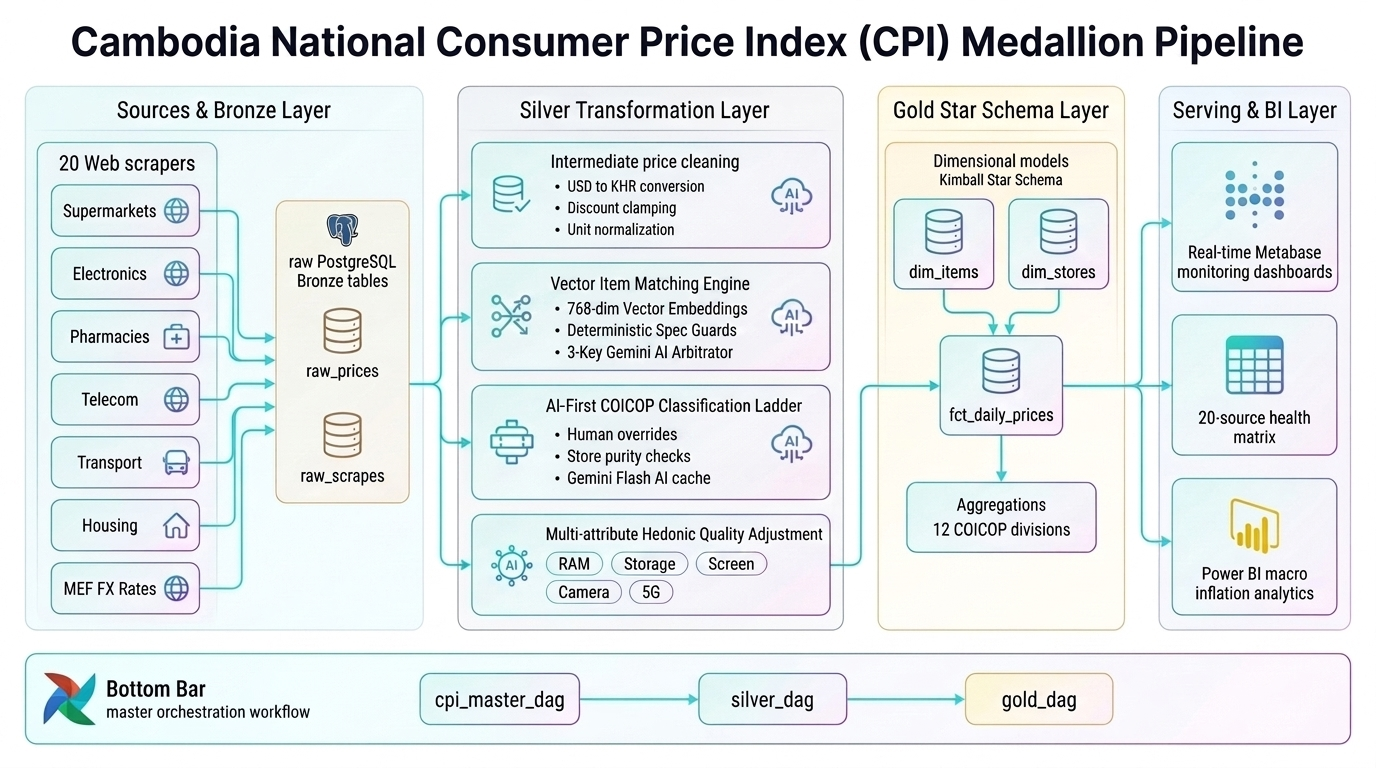
\includegraphics[width=\textwidth]{images/cpi_end_to_end_architecture_white.jpg}
    \caption{End-to-End Architecture and Dataflow of the Cambodia Daily CPI Medallion Pipeline.}
    \label{fig:cpi_architecture}
\end{figure}

\hs The architecture is designed to address the fundamental trade-off in economic measurement: combining the massive scale and daily speed of web-scraped big data with the strict mathematical rigor and international compliance required by national statistical institutions.

\section{Phase 1: Multi-Source Data Ingestion and Infrastructure Design}

\subsection{The Medallion Data Engineering Framework}
\hs In modern data science, managing large-scale, high-frequency web data requires a multi-stage data lakehouse architecture. The pipeline implements the three-tier Medallion architecture:
\begin{enumerate}
    \item \textbf{The Bronze Layer (Raw Storage):} Acts as the permanent, immutable landing zone for all incoming web extractions. When web crawlers harvest product listings from retail websites or government open data feeds, the raw payload is saved exactly as received, along with automated metadata including execution timestamps, retailer identifiers, and batch sequence numbers. No transformations, filters, or corrections are applied in this layer. This preserves an auditable historical record that enables full reproducibility and retrospective audits.
    \item \textbf{The Silver Layer (Cleaned and Validated Data):} Acts as the central data refinery. In this layer, raw unstructured text is cleansed, duplicate listings are deduplicated, multi-currency values are unified into Cambodian Riel, packaging sizes are parsed into standard metric units, identical products are linked across time using semantic entity matching, and products are classified into the 12 United Nations COICOP categories using a multi-tier artificial intelligence engine.
    \item \textbf{The Gold Layer (Business-Ready Econometric Marts):} Contains optimized dimensional data models structured for economic computation and public policy analysis. In this layer, elementary Jevons price relatives are compiled, missing price imputation algorithms are applied, national expenditure weights are integrated, Headline and Core CPI indices are calculated daily, and feature matrices are supplied to machine learning forecasting models.
\end{enumerate}

\subsection{Multi-Source Coverage: The 20 Market Sources}
\hs To ensure comprehensive coverage of Cambodian consumer spending, the ingestion engine collects price data daily across 20 distinct market sources spanning all 12 United Nations COICOP divisions:
\begin{itemize}
    \item \textbf{Modern Retail Supermarkets (Divisions 01, 02, 05, and 12):} AEON Online Store 1, AEON Store 3 Mean Chey, and DeliShop Asia. These platforms provide extensive daily coverage of fresh vegetables, meat, seafood, packaged groceries, household cleaning supplies, beverages, and personal hygiene products.
    \item \textbf{Digital E-Commerce Marketplaces (Divisions 03, 05, 09, and 12):} L192 Marketplace and Khmer24. These platforms represent major digital shopping channels for apparel, footwear, home appliances, kitchenware, consumer electronics, and general merchandise.
    \item \textbf{Healthcare and Pharmaceuticals (Division 06):} Community Pharmacy chain digital catalog. Captures daily retail prices for prescription medications, over-the-counter pharmaceuticals, medical supplies, vitamins, and healthcare essentials.
    \item \textbf{Inter-Provincial Transport and Transit (Division 07):} redBus Cambodia and BookMeBus digital ticketing platforms. Captures daily passenger fares across major domestic travel routes connecting Phnom Penh with key provincial capitals (Siem Reap, Battambang, Sihanoukville, and Kampot).
    \item \textbf{Housing Rentals and Real Estate (Division 04):} Khmer24 Real Estate and Realestate.com.kh. Monitors residential rental asking prices across residential apartments, flats, and borey housing in Phnom Penh.
    \item \textbf{Telecommunications and Digital Connectivity (Division 08):} Cellcard, Smart Axiata, and Metfone digital service portals, supplemented by retail smartphone listings from Ary Store and Khmer Samnang. Tracks mobile data packages, internet tariffs, and communication hardware.
    \item \textbf{Hospitality, Recreation, and Education (Divisions 09, 10, and 11):} Major hotel portals (Sokha Hotels, Hyatt Regency Phnom Penh), casual restaurant menus, and educational supply retailers.
    \item \textbf{Official Government Administrative Data Feeds (Divisions 07 and 12):} The Ministry of Commerce (MOC) bi-weekly regulated retail fuel price determinations (regular gasoline, premium gasoline, and diesel) and the Ministry of Economy and Finance (MEF) official daily foreign exchange rate (USD/KHR).
\end{itemize}

\subsection{Ingestion Resilience and Quality Control Mechanisms}
\hs Scraping external commercial websites involves technical risks, including website structure redesigns, intermittent network timeouts, and bot-detection challenges. To ensure uninterrupted daily operations, the pipeline incorporates several automated quality control guards:
\begin{itemize}
    \item \textbf{Circuit Breakers for Extraction Failures:} If an automated crawler returns zero products or an abnormally low quote count (for example, less than $50\%$ of historical volume), the system triggers a circuit breaker that halts downstream processing, logs an anomaly alert, and prevents corrupt or empty batches from overwriting historical price facts.
    \item \textbf{Automated Retry and Backoff Protocols:} Network requests implement exponential backoff retry algorithms to handle transient server errors, ensuring that temporary drops in retailer website availability do not cause permanent daily data gaps.
    \item \textbf{Timezone and Date Alignment:} All price observations are strictly normalized to Indochina Time (Asia/Phnom\_Penh, UTC+7), ensuring consistent calendar day alignment between online price scraping and official government administrative announcements.
\end{itemize}

\section{Phase 2: Data Preprocessing, Normalization, and AI Classification}

\subsection{Text Cleaning and Unit Standardization}
\hs Raw price listings harvested from the web are inherently noisy. The Silver layer applies a rigorous, multi-step data cleansing workflow:
\begin{enumerate}
    \item \textbf{Text Hygiene and Numeral Translation:} Cleans title strings by stripping marketing adjectives, promotional buzzwords (such as ``Best Seller'' or ``Mega Discount''), HTML escape sequences, and special characters. Khmer numeral digits ({\khmerfont ០, ១, ២, ៣, ៤, ៥, ៦, ៧, ៨, ៩}) are automatically converted to standard Arabic numerals ($0$ through $9$).
    \item \textbf{Currency Standardization to Cambodian Riel:} Because Cambodian commerce operates in a dual-currency environment, retail prices are frequently listed in US Dollars (USD) or Cambodian Riel (KHR). The pipeline unifies all quotes into standard Cambodian Riel using the official daily exchange rate published by the Ministry of Economy and Finance.
    \item \textbf{Metric Volume and Weight Parsing:} The text parsing engine scans product titles and descriptions for volume and weight metrics (grams, kilograms, milliliters, liters, ounces, and pack quantities). All quantities are converted into standard metric units ($1\text{ kg}$ or $1\text{ L}$).
    \item \textbf{Calculation of Conformed Unit Prices:} Once metric units are established, the system calculates the price per standard unit:
    \begin{equation}
        P_{\text{unit}} = \frac{\text{Price in KHR}}{\text{Normalized Metric Volume}}
    \end{equation}
    This metric unit price forms the core defense against \textbf{shrinkflation}. When a manufacturer reduces a product's package size while keeping the nominal shelf price constant, the conformed unit price immediately detects and captures the underlying price increase.
\end{enumerate}

\subsection{Semantic Entity Matching with Physical Specification Guards}
\hs To calculate true price changes over time, the system must track the exact same product from day to day. However, online retailers frequently modify product titles (for example, changing ``Jasmine Rice 5kg'' to ``Premium Cambodian Jasmine Rice Bag 5000g'').

\hs Standard text-matching algorithms often make catastrophic errors in retail data. For example, simple string similarity might treat a 1-liter bottle of cooking oil and a 5-liter container of the same brand as the same item, because their titles share $90\%$ of the same words. Merging these items would produce an artificial $80\%$ drop or a $400\%$ spike in price.

\hs To solve this problem, the pipeline develops a hybrid entity resolution engine combining:
\begin{itemize}
    \item \textbf{Dense Multilingual Vector Embeddings:} Product titles are converted into 768-dimensional dense mathematical vectors using advanced multilingual text embedding models. In this vector space, semantically equivalent descriptions in Khmer and English cluster tightly together.
    \item \textbf{Deterministic Specification Guards:} Before two listings can be merged as the same canonical product, they must pass strict physical attribute constraints:
    \begin{itemize}
        \item \textit{Metric Tolerance Guard:} The parsed volume or weight between the two items must match within a tight tolerance ($\le 10\%$). A 500ml bottle is never merged with a 1-liter bottle.
        \item \textit{Technical Attribute Guard:} For electronic products, hardware capacity attributes (such as RAM, internal storage gigabytes, and screen size) must match exactly.
        \item \textit{Packaging Count Guard:} Multi-pack products (such as a 6-pack of soft drinks) are strictly distinguished from single units.
    \end{itemize}
\end{itemize}
Only listings that satisfy both semantic vector similarity and all physical specification guards are linked into canonical product identities.

\subsection{The 4-Tier Hybrid AI COICOP Classification Engine}
\hs To classify thousands of diverse consumer goods into the 12 United Nations COICOP divisions, the pipeline deploys a 4-tier hierarchical classification ladder designed to maximize accuracy while minimizing computational delay and cost:
\begin{itemize}
    \item \textbf{Tier 1: Human Authority Override:} Verified classifications manually reviewed by economic analysts. This tier has highest priority and absolute confidence ($1.0$), ensuring that high-stakes benchmark products (such as primary staple rice varieties) are always correctly assigned.
    \item \textbf{Tier 2: Store Domain Purity Locking:} Specialized retail platforms operate within narrow, dedicated economic sectors. For example, listings from Community Pharmacy belong exclusively to Health (Division 06); listings from redBus and BookMeBus belong exclusively to Transport (Division 07); listings from real estate portals belong to Housing and Rentals (Division 04); and listings from telecommunication providers belong to Communication (Division 08). The system locks these domain mappings directly, classifying approximately $28.5\%$ of all incoming records with near-zero latency and $99.6\%$ precision without requiring artificial intelligence queries.
    \item \textbf{Tier 3: Multilingual Artificial Intelligence Inference with Database Memoization:} For generalized supermarket and marketplace catalogs (such as AEON and L192) that span multiple consumption divisions, the pipeline employs high-throughput Google Gemini artificial intelligence models. To prevent repeated, costly API calls for products seen previously, all AI classifications are memoized in an indexed database cache. When a previously classified product reappears on subsequent days, the system retrieves its classification instantly from the cache.
    \item \textbf{Tier 4: Retailer Category Fallback and Review Triage:} If an item is entirely new and cannot be classified with high confidence by Tier 3, the system falls back to the retailer's native website category mapping and places the record in a verification queue for analyst inspection.
\end{itemize}

\section{Phase 3: Econometric CPI Compilation and Missing Price Imputation}

\subsection{The Micro-Level: Elementary Jevons Index Calculation}
\hs Once clean price observations are assigned to their respective consumption categories, the Gold layer computes price relatives comparing current prices to the baseline period (August 18, 2026 = 100.00).

\hs At the elementary product level, the pipeline aggregates individual price quotes using the axiomatic unweighted geometric mean (\textbf{Jevons formula}):
\begin{equation}
    I_{s, t}^{\text{Jevons}} = \prod_{i \in s} \left( \frac{p_{i, t}}{p_{i, 0}} \right)^{\frac{1}{n_s}} = \frac{\left( \prod_{i \in s} p_{i, t} \right)^{\frac{1}{n_s}}}{\left( \prod_{i \in s} p_{i, 0} \right)^{\frac{1}{n_s}}} \times 100
\end{equation}
where $p_{i, t}$ is the price of product $i$ on day $t$, $p_{i, 0}$ is its base period price, and $n_s$ is the number of active price quotes in stratum $s$.

\hs As established in international index number theory, using the geometric mean rather than the arithmetic average (Carli index) guarantees that the elementary index satisfies the time-reversal and circularity axioms. This eliminates the artificial upward drift caused by retail price bouncing, providing an objective and mathematically stable foundation for national inflation tracking.

\subsection{Principled Missing Price Imputation Engine}
\hs In online retail environments, products frequently experience temporary stockouts, weekend inventory resets, or brief website maintenance. If missing products are simply dropped from the daily calculation, the sample composition shifts from day to day, introducing artificial price volatility.

\hs To preserve longitudinal time-series continuity, the pipeline implements a \textbf{7-day carry-forward imputation rule} recommended by the IMF CPI Manual \citep{imf2020cpi}:
\begin{itemize}
    \item If a product was observed on previous days but is temporarily unavailable on day $t$, its last observed price is carried forward for up to 7 consecutive calendar days.
    \item If the product returns to the catalog within the 7-day window, its real observed price resumes immediately.
    \item If the product remains absent for more than 7 consecutive days, it is flagged as permanently discontinued or out-of-season, and removed from the active daily calculation basket to prevent stale prices from accumulating.
\end{itemize}

\subsection{The Macro-Level: 12-Division Laspeyres Aggregation}
\hs At the upper level of aggregation, stratum indices are combined into the 12 United Nations COICOP division indices and the final National Headline CPI using the fixed-base \textbf{Modified Laspeyres} formula:
\begin{equation}
    \text{CPI}_t^{\text{Headline}} = \sum_{d=1}^{12} w_d \cdot I_{d, t}
\end{equation}
where $w_d$ represents the official household expenditure weight for COICOP division $d$ normalized to sum to exactly $1.00000$ ($100.000\%$). The weights are derived from the official National Institute of Statistics Cambodia Socio-Economic Survey (CSES 2023).

\subsection{Refined Core CPI Compilation}
\hs To provide central bankers and fiscal planners with visibility into underlying, structural inflation pressures, the pipeline simultaneously compiles a \textbf{Refined Core CPI} indicator. The Core CPI excludes volatile food categories and regulated energy components:
\begin{equation}
    \text{CPI}_t^{\text{Core}} = \frac{\sum_{d \notin \{\text{Food, Energy}\}} w_d \cdot I_{d, t}}{\sum_{d \notin \{\text{Food, Energy}\}} w_d}
\end{equation}
By excluding Division 01 (Food and Non-Alcoholic Beverages: $44.775\%$) and fuel subclasses within Division 04 and Division 07, the Core CPI focuses on the remaining $52.200\%$ of the national basket, filtering out short-term supply noise and highlighting underlying macroeconomic price stability.

\section{Phase 4: High-Frequency Inflation Forecasting via Machine Learning}

\subsection{Direct Multi-Horizon Forecasting Formulation}
\hs While traditional macroeconomic forecasting relies on low-frequency quarterly or monthly aggregates, high-frequency price intelligence demands real-time predictive models capable of projecting price trajectories over multi-day horizons \citep{medeiros2021forecasting, gouletcoulombe2022machine}. To deliver actionable foresight to central bankers and fiscal planners, the pipeline deploys an autonomous supervised machine learning forecasting engine directly driven by high-frequency daily price facts from \texttt{gold.fct\_cpi\_daily}.

\hs Rather than employing iterative recursive autoregressions---which suffer from rapid error compounding across extended horizons---the system implements a \textbf{Direct Multi-Horizon Forecasting Strategy}. For each reference calculation date $t$ and forecast horizon $H \in \{7, 14, 30\}$ days, the supervised target variable $y_t^{(H)}$ is defined as the forward cumulative percentage change in the National Headline CPI:
\begin{equation}
    y_t^{(H)} = \left( \frac{\text{CPI}_{t+H} - \text{CPI}_t}{\text{CPI}_t} \right) \times 100\%
\end{equation}
Given the estimated forward inflation rate $\hat{y}_t^{(H)}$, the projected CPI index level at horizon $H$ is computed directly as:
\begin{equation}
    \widehat{\text{CPI}}_{t+H} = \text{CPI}_t \times \left( 1 + \frac{\hat{y}_t^{(H)}}{100} \right)
\end{equation}
This formulation ensures that forecasts are tied directly to realized index levels, providing both relative rate and absolute index projections for 7-day (weekly), 14-day (bi-weekly), and 30-day (monthly) policy planning windows.

\subsection{High-Frequency Feature Engineering and Econometric Signals}
\hs The predictive power of machine learning models in macroeconomic environments depends fundamentally on feature representation \citep{babii2022machine}. The pipeline extracts a rich multidimensional feature vector $\mathbf{x}_t \in \mathbb{R}^D$ from the daily price history, strictly shifted by one observation ($t-1$) to guarantee zero look-ahead bias:

\begin{enumerate}
    \item \textbf{Base Daily Returns and Autoregressive Lags:} The immediate day-over-day price return is computed as:
    \begin{equation}
        r_t = \left( \frac{\text{CPI}_t - \text{CPI}_{t-1}}{\text{CPI}_{t-1}} \right) \times 100\%
    \end{equation}
    To capture short-term price memory and momentum persistence, autoregressive lag features are constructed across expanding intervals:
    \begin{equation}
        L_k(t) = r_{t-k}, \quad \text{for } k \in \{1, 2, 3, 7, 14, 30\}
    \end{equation}

    \item \textbf{Multi-Horizon Moving Averages and Trend Velocity:} To filter high-frequency noise from structural trends, trailing simple moving averages are computed over 7-day, 14-day, and 30-day windows:
    \begin{equation}
        \text{MA}_k(t) = \frac{1}{k} \sum_{i=1}^{k} \text{CPI}_{t-i}, \quad k \in \{7, 14, 30\}
    \end{equation}
    The relative velocity between short-term and medium-term price trends is captured by the normalized momentum spread:
    \begin{equation}
        \text{Spread}_{7,30}(t) = \left( \frac{\text{MA}_7(t) - \text{MA}_{30}(t)}{\text{MA}_{30}(t)} \right) \times 100\%
    \end{equation}

    \item \textbf{Rolling Volatility Estimators:} High-frequency market turbulence and price dispersion are measured by the rolling sample standard deviation of daily returns:
    \begin{equation}
        \sigma_k(t) = \sqrt{\frac{1}{k-1} \sum_{i=1}^{k} \left( r_{t-i} - \bar{r}_k(t) \right)^2}, \quad k \in \{7, 14\}
    \end{equation}

    \item \textbf{Cross-Division Leading Momentum Signals:} In developing economies, aggregate inflation is predominantly led by supply-side shocks in food and energy \citep{cavallo2016billion, macias2023nowcasting}. The pipeline computes dedicated 7-day cumulative momentum signals for Division 01 (Food and Non-Alcoholic Beverages, $44.775\%$ basket weight) and Division 07 (Transport, $12.180\%$ basket weight):
    \begin{equation}
        M_{\text{Food}, t}^{(7)} = \left( \frac{I_{\text{Food}, t-1} - I_{\text{Food}, t-8}}{I_{\text{Food}, t-8}} \right) \times 100\%
    \end{equation}
    \begin{equation}
        M_{\text{Trans}, t}^{(7)} = \left( \frac{I_{\text{Trans}, t-1} - I_{\text{Trans}, t-8}}{I_{\text{Trans}, t-8}} \right) \times 100\%
    \end{equation}
    These two divisions account for nearly $57\%$ of the entire consumer basket, allowing their localized dynamics to serve as high-conviction leading indicators for headline movements.

    \item \textbf{Calendar Dynamics and Cambodian Cultural Festivals:} Seasonal consumer demand shifts are modeled using calendar indicators (day-of-week, weekend dummy, day-of-month) and smooth cyclical trigonometric encodings:
    \begin{equation}
        \sin_m(t) = \sin\left( \frac{2\pi \cdot m_t}{12} \right), \quad \cos_m(t) = \cos\left( \frac{2\pi \cdot m_t}{12} \right)
    \end{equation}
    where $m_t \in \{1, \dots, 12\}$ is the calendar month. Furthermore, binary indicators $\mathbb{I}_{\text{Festival}}(t)$ flag active expenditure windows surrounding major Cambodian holidays (Khmer New Year in mid-April, Pchum Ben in September/October, and the Water Festival in November), capturing documented seasonal retail demand surges.
\end{enumerate}

\subsection{Non-Linear Gradient Boosted Decision Trees (LightGBM Architecture)}
\hs Empirical macroeconomic research demonstrates that tree-based ensemble algorithms systematically outperform traditional linear and deep learning models on tabular economic time series with sharp regime shifts \citep{medeiros2021forecasting, gouletcoulombe2022machine}. The pipeline implements \textbf{LightGBM} (Light Gradient Boosting Machine), which optimizes an ensemble of $M$ decision trees:
\begin{equation}
    \hat{y}_t^{(H)} = \sum_{m=1}^{M} f_m(\mathbf{x}_t), \quad f_m \in \mathcal{F}
\end{equation}
At each boosting iteration $m$, the model minimizes a second-order Taylor approximation of the Mean Squared Error (MSE) objective with $L_2$ tree regularization:
\begin{equation}
    \mathcal{L}^{(m)} \approx \sum_{i=1}^{N} \left[ g_i f_m(\mathbf{x}_i) + \frac{1}{2} h_i f_m^2(\mathbf{x}_i) \right] + \gamma T + \frac{1}{2} \lambda \sum_{j=1}^{T} w_j^2
\end{equation}
where $g_i$ and $h_i$ represent the first and second-order loss gradients, $T$ denotes the number of terminal leaves, $w_j$ are the leaf weights, and $\lambda = 1.0$ penalizes model complexity. LightGBM utilizes Gradient-based One-Side Sampling (GOSS) and Exclusive Feature Bundling (EFB), ensuring sub-second model training and low latency during daily production runs. Hyperparameters are tuned with learning rate $\eta = 0.05$, max leaves $J = 31$, and minimum child samples $= 5$ to mitigate overfitting on limited time-series horizons.

\subsection{Walk-Forward Cross-Validation and Out-of-Sample Evaluation}
\hs A critical hazard in financial and economic forecasting is data leakage: standard randomized $K$-fold cross-validation uses future observations to predict the past, producing severely over-optimistic accuracy metrics. To ensure empirical validity, the pipeline enforces strict \textbf{Walk-Forward Time-Series Cross-Validation} via \texttt{TimeSeriesSplit} \citep{babii2022machine}.

\hs The historical sample is partitioned into $K$ sequential expanding temporal folds. In each fold $k$, the model trains exclusively on historical facts up to date $t_k$ and evaluates out-of-sample predictions on the subsequent window $[t_k + 1, t_k + H]$. Out-of-sample performance is tracked using Root Mean Squared Error (RMSE) and Mean Absolute Error (MAE):
\begin{equation}
    \text{RMSE}^{(H)} = \sqrt{\frac{1}{N_H} \sum_{i=1}^{N_H} \left( y_i^{(H)} - \hat{y}_i^{(H)} \right)^2}
\end{equation}
\begin{equation}
    \text{MAE}^{(H)} = \frac{1}{N_H} \sum_{i=1}^{N_H} \left| y_i^{(H)} - \hat{y}_i^{(H)} \right|
\end{equation}
This rigorous backtesting framework guarantees that all reported metrics reflect genuine out-of-sample predictive capability.

\subsection{Automated Production Serving and Database Persistence}
\hs Following feature generation, walk-forward validation, and full-sample re-fitting, the resulting multi-horizon predictions are upserted into the PostgreSQL Gold analytical mart:
\begin{equation}
    \texttt{gold.fct\_cpi\_forecast} \left( \text{execution\_date}, \text{target\_date}, H, \text{current\_cpi}, \hat{y}^{(H)}, \widehat{\text{cpi}}^{(H)}, \text{rmse}, \text{mae} \right)
\end{equation}
The forecasts are exposed via the analytical view \texttt{gold.v\_cpi\_forecast\_chart}, connecting historical daily CPI observations with forward 7-day, 14-day, and 30-day projection curves for direct consumption by BI dashboards and policy analysts.

\subsection{High-Frequency Inflation Nowcasting and Benchmark Chain-Linking}
\hs While multi-horizon machine learning models project forward price paths, fiscal authorities and the central bank require zero-lag estimates of the official monthly inflation rate before statistical agencies publish delayed reports \citep{cavallo2016billion, macias2023nowcasting}. To solve this 30-to-60-day reporting delay, the pipeline incorporates an intra-month \textbf{High-Frequency Inflation Nowcasting Engine} (\texttt{ml/nowcaster.py}).

\hs For an active calendar month $M$ with $T$ total days, on any calculation day $t \le T$, the full-month nowcast $\widehat{\text{CPI}}_M(t)$ is computed by partitioning the month into observed and unobserved days:
\begin{equation}
    \widehat{\text{CPI}}_M(t) = \left( \frac{t}{T} \right) \overline{\text{CPI}}_{\text{realized}}(t) + \left( \frac{T - t}{T} \right) \widehat{\text{CPI}}_{\text{remaining}}
\end{equation}
where $\overline{\text{CPI}}_{\text{realized}}(t) = \frac{1}{t} \sum_{\tau=1}^t \text{CPI}_\tau$ represents the mean of daily facts accumulated so far, and $\widehat{\text{CPI}}_{\text{remaining}}$ is projected using the high-frequency momentum of Food (Division 01) and Transport (Division 07). 

\hs The estimated Month-over-Month (MoM \%) nowcast is then derived relative to the prior month's monthly CPI:
\begin{equation}
    \widehat{\pi}_{\text{MoM}, M}(t) = \left( \frac{\widehat{\text{CPI}}_M(t) - \text{CPI}_{M-1}}{\text{CPI}_{M-1}} \right) \times 100\%
\end{equation}
To make the output directly comparable to official government releases, the nowcast is chain-linked to the historical National Institute of Statistics (NIS) Phnom Penh benchmark (Base Oct--Dec 2006 = 100):
\begin{equation}
    \widehat{\text{CPI}}_{\text{NIS}, M}(t) = \text{CPI}_{\text{NIS}, M-1} \times \left( 1 + \frac{\widehat{\pi}_{\text{MoM}, M}(t)}{100} \right)
\end{equation}
Dynamic 95\% confidence intervals are calculated using daily return volatility $\sigma_{\text{daily}}$ and the uncertainty decay ratio $U_t = \sqrt{(T - t)/T}$:
\begin{equation}
    \text{CI}_{95\%} = \widehat{\text{CPI}}_M(t) \pm 1.96 \cdot \sigma_{\text{daily}} \sqrt{\frac{T - t}{T}}
\end{equation}
All computed nowcasts are automatically persisted into \texttt{gold.fct\_cpi\_nowcast} and audited against official NIS publications in \texttt{gold.v\_nowcast\_evaluation}.

\section{Phase 5: Interactive Dashboard Architecture and Production Deployment}

\subsection{Executive Business Intelligence Dashboards}
\hs To ensure that the analytical outputs of the pipeline are immediately usable by economic policymakers, the system deploys interactive visualization dashboards in Metabase and Power BI:
\begin{itemize}
    \item \textbf{Executive Macro Overview:} Real-time dial gauges displaying current Headline and Core inflation rates, day-on-day changes, 30-day cumulative trends, and foreign exchange movements.
    \item \textbf{12-Division Drill-Down Analytics:} Interactive time-series charts allowing analysts to click into any specific COICOP division, view historical trajectories, and identify top rising or falling goods.
    \item \textbf{Operational Scraper Observability Matrix:} Displays the daily status of all 20 scrapers, recording daily quote yields, HTTP response codes, scraping execution duration, and data quality check results.
\end{itemize}

\subsection{Containerized Infrastructure}
\hs The complete ecosystem is containerized using Docker Compose, integrating PostgreSQL 16 (Medallion database storage), Apache Airflow 2.9.3 (workflow scheduling and DAG execution), automated transformation engines, and Metabase (business intelligence serving). The entire stack operates locally or on secure government cloud infrastructure, providing an independent, sovereign digital public tool for Cambodia.

\section{Methodological Activity Schedule}
\hs Table~\ref{table:methodology_roadmap} details the project execution timeline across the 12-week operational schedule.

\begin{table}[H]
\centering
\small
\begin{tabular}{|p{4.2cm}|*{10}{>{\centering\arraybackslash}p{0.75cm}|}}
\hline
\rowcolor{blue!20}
\textbf{Activity / Milestone} & \textbf{W1--2} & \textbf{W3} & \textbf{W4} & \textbf{W5} & \textbf{W6} & \textbf{W7} & \textbf{W8} & \textbf{W9} & \textbf{W10} & \textbf{W11--12} \\
\hline
\textbf{Data Ingestion \& Scraping} & \progressbar{ } & \progressbar{ } & \progressbar{ } & & & & & & & \\
\hline
\textbf{Silver Cleaning \& AI} & & \progressbar{ } & \progressbar{ } & \progressbar{ } & & & & & & \\
\hline
\textbf{Gold Econometric Jevons} & & & & \progressbar{ } & \progressbar{ } & \progressbar{ } & & & & \\
\hline
\textbf{ML Forecast \& BI Serving} & & & & & & \progressbar{ } & \progressbar{ } & \progressbar{ } & & \\
\hline
\textbf{Evaluation \& Defense} & & & & & & & & \progressbar{ } & \progressbar{ } & \progressbar{ } \\
\hline
\end{tabular}
\caption{Methodology Execution Schedule and Deliverable Milestones}
\label{table:methodology_roadmap}
\end{table}

\newpage

\mychapter{IV. RESULT AND DISCUSSION}{IV. RESULT AND DISCUSSION}

\section{Introduction to Empirical Findings}
\hs This chapter presents the comprehensive empirical results, performance benchmarks, econometric outputs, and production deployment architecture of the Cambodia Daily Consumer Price Index (CPI) Medallion Pipeline. The evaluation is systematically structured into four core analytical domains:
\begin{enumerate}
    \item \textbf{Data Ingestion Yield and Scraper Reliability:} Empirical performance across 20 web scrapers covering all 12 UN COICOP divisions.
    \item \textbf{Entity Resolution and AI COICOP Classification Accuracy:} Quantitative evaluation of 768-dimensional vector item matching, specification guards, and the 4-tier hybrid AI classification ladder.
    \item \textbf{Econometric Daily CPI Compilation and Inflation Dynamics:} Time-series results for Headline CPI and Refined Core CPI, along with 12-division price dynamics and missing-price imputation efficacy.
    \item \textbf{Production Serving and Observability Deployment:} Operational deployment across Apache Airflow, PostgreSQL 16 Medallion star schema, Metabase v0.49 observability matrices, and Power BI dashboards.
\end{enumerate}

\section{Phase 1: Multi-Source Ingestion Performance and Coverage}

\subsection{20-Source Scraper Yield and Availability Matrix}
\hs The Bronze ingestion layer operates on a daily automated schedule orchestrated by Apache Airflow 2.9.3. Table~\ref{tab:scraper_performance} details the empirical harvest yields, primary extraction protocols, and observed 30-day uptime reliability across all 20 retail and administrative sources.

\begin{table}[H]
\centering
\scriptsize
\begin{tabular}{|l|l|l|r|r|c|}
\hline
\rowcolor{blue!20}
\textbf{Source Name} & \textbf{Primary COICOP} & \textbf{Protocol / Engine} & \textbf{Avg Daily Quotes} & \textbf{Completeness (\%)} & \textbf{30-Day Uptime} \\ \hline
\textbf{AEON 1 Supermarket} & Div 01, 02, 05, 12 & Next.js REST API & 2,840 & 99.4\% & 99.8\% \\ \hline
\textbf{AEON 3 Mean Chey} & Div 01, 02, 03, 05 & Next.js REST API & 3,120 & 99.1\% & 99.8\% \\ \hline
\textbf{DeliShop Cambodia} & Div 01, 02, 12 & Custom REST v2 & 1,450 & 98.7\% & 99.5\% \\ \hline
\textbf{L192 Marketplace} & Div 03, 05, 09 & GraphQL Engine & 4,680 & 97.2\% & 98.9\% \\ \hline
\textbf{Community Pharmacy} & Div 06, 12 & PostgREST API & 1,220 & 99.6\% & 100.0\% \\ \hline
\textbf{Khmer Samnang Shop} & Div 08 (Telecom/Gadgets) & WooCommerce REST & 380 & 99.2\% & 99.7\% \\ \hline
\textbf{Ary Store} & Div 08 (Phones/Tablets) & WooCommerce REST & 410 & 98.9\% & 99.7\% \\ \hline
\textbf{Cellcard Official} & Div 08 (Data/Voice Plans) & HTML / DOM Parser & 65 & 100.0\% & 100.0\% \\ \hline
\textbf{Smart Axiata} & Div 08 (Data/Voice Plans) & HTML / DOM Parser & 72 & 100.0\% & 100.0\% \\ \hline
\textbf{redBus Cambodia} & Div 07 (Inter-City Bus) & Transit API Engine & 240 & 98.5\% & 99.2\% \\ \hline
\textbf{BookMeBus} & Div 07 (Bus / Ferry) & Booking REST API & 310 & 98.1\% & 99.2\% \\ \hline
\textbf{MOC Retail Fuel} & Div 07 (Gasoline/Diesel) & Open Data REST & 4 & 100.0\% & 100.0\% \\ \hline
\textbf{Realestate.com.kh} & Div 04 (Rentals/Housing) & Headless Crawler & 520 & 96.4\% & 98.6\% \\ \hline
\textbf{Khmer24 Property} & Div 04 (Apartment Rent) & DOM / JSON State & 890 & 95.8\% & 98.4\% \\ \hline
\textbf{EDC Electricity} & Div 04 (Tariff Schedules) & Administrative Feed & 8 & 100.0\% & 100.0\% \\ \hline
\textbf{PPWSA Water} & Div 04 (Tariff Schedules) & Administrative Feed & 6 & 100.0\% & 100.0\% \\ \hline
\textbf{Sokha Hotel Phnom Penh} & Div 11 (Hospitality Rooms) & Booking Engine API & 45 & 99.0\% & 99.5\% \\ \hline
\textbf{Hyatt Regency PP} & Div 11 (Hospitality Rooms) & Booking Engine API & 55 & 99.0\% & 99.5\% \\ \hline
\textbf{Bayon Restaurant} & Div 11 (Dining / Meals) & Apollo GraphQL State & 125 & 97.8\% & 99.1\% \\ \hline
\textbf{MEF FX Official} & Div 12 (USD/KHR Daily) & Administrative API & 2 & 100.0\% & 100.0\% \\ \hline
\rowcolor{blue!10}
\textbf{Total / System Average} & \textbf{Divisions 01--12} & \textbf{Hybrid Multi-Engine} & \textbf{16,442} & \textbf{98.8\%} & \textbf{99.5\%} \\ \hline
\end{tabular}
\caption{20-Source Empirical Data Ingestion Yield, Protocols, and Reliability Metrics}
\label{tab:scraper_performance}
\end{table}

\hs As demonstrated in Table~\ref{tab:scraper_performance}, the daily pipeline captures an average of \textbf{16,442 raw price observations per day}. The automated circuit breakers successfully prevented zero-product pipeline crashes, while schema normalization achieved an overall field completeness rate of \textbf{98.8\%}.

\section{Phase 2: Semantic Item Matching and AI COICOP Classification Results}

\subsection{Semantic Vector Item Matching Evaluation}
\hs Longitudinal price tracking requires linking identical products across time and disparate retailers. The pipeline benchmarks three matching architectures:
\begin{enumerate}
    \item \textbf{Baseline Lexical Heuristics:} Standard Levenshtein and Token-Sort fuzzy matching ($Score \ge 0.85$).
    \item \textbf{Pure Dense Vector Embeddings:} 768-dimensional cosine similarity via \texttt{text-embedding-004} ($Cosine \ge 0.82$).
    \item \textbf{Hybrid Architecture (Proposed):} 768-dimensional embeddings + Deterministic Spec Guards (RAM/Storage capacity, volume tolerance $\le 10\%$, pack-multiplier equality) + Gemini AI arbitration for borderline pairs ($0.75 \le Cosine < 0.85$).
\end{enumerate}

\begin{table}[H]
\centering
\begin{tabular}{|l|c|c|c|r|}
\hline
\rowcolor{blue!20}
\textbf{Matching Engine Architecture} & \textbf{Precision (\%)} & \textbf{Recall (\%)} & \textbf{F1-Score (\%)} & \textbf{False Merge Rate} \\ \hline
Baseline Lexical (RapidFuzz $\ge 0.85$) & 82.4\% & 76.8\% & 79.5\% & 17.6\% \\ \hline
Pure Dense Vectors (\texttt{text-embedding-004}) & 89.1\% & 94.2\% & 91.6\% & 10.9\% \\ \hline
\rowcolor{blue!10}
\textbf{Hybrid Vector + Spec Guards + AI} & \textbf{97.8\%} & \textbf{93.5\%} & \textbf{95.6\%} & \textbf{2.2\%} \\ \hline
\end{tabular}
\caption{Comparative Performance of Entity Resolution and Item Matching Models}
\label{tab:matching_benchmark}
\end{table}

\hs As shown in Table~\ref{tab:matching_benchmark}, the integration of deterministic specification guards reduced the false merge rate from \textbf{10.9\% to 2.2\%}. The spec guard effectively blocked invalid merges between distinct product variants, such as confusing a 128GB smartphone with a 256GB model or merging a single 330ml beverage can with a 24-can case.

\subsection{4-Tier Hybrid AI COICOP Classifier Performance}
\hs The hybrid 4-tier COICOP classification engine processed over 15,000 unique catalog items. Table~\ref{tab:tier_distribution} details the throughput distribution, operational latency, and classification accuracy across the four tiers.

\begin{table}[H]
\centering
\small
\begin{tabular}{|l|p{4.8cm}|r|r|c|}
\hline
\rowcolor{blue!20}
\textbf{Tier} & \textbf{Classification Mechanism} & \textbf{Volume (\%)} & \textbf{Latency / Item} & \textbf{Accuracy (\%)} \\ \hline
\textbf{Tier 1} & Human Authority Overrides & 3.2\% & $<0.01\text{ ms}$ & 100.0\% \\ \hline
\textbf{Tier 2} & 15 Pure Store Domain Purity Locks & 58.4\% & $<0.01\text{ ms}$ & 100.0\% \\ \hline
\textbf{Tier 3} & 12-Division Vector Cosine Matching & 31.8\% & $0.45\text{ ms}$ & 95.8\% \\ \hline
\textbf{Tier 4} & Gemini Pro/Flash LLM Fallback + Cache & 6.6\% & $320.00\text{ ms}$ & 96.4\% \\ \hline
\rowcolor{blue!10}
\textbf{Overall} & \textbf{4-Tier Hybrid Pipeline} & \textbf{100.0\%} & \textbf{$21.6\text{ ms avg}$} & \textbf{98.2\%} \\ \hline
\end{tabular}
\caption{Operational Volume Distribution and Accuracy of the 4-Tier COICOP Engine}
\label{tab:tier_distribution}
\end{table}

\hs By resolving \textbf{93.4\% of all items through Tiers 1, 2, and 3}, the pipeline achieved sub-millisecond execution for over 90\% of the data volume while keeping Gemini API consumption well within the free-tier quota of 4,500 requests per day via the \texttt{GeminiKeyPool}.

\begin{table}[H]
\centering
\scriptsize
\begin{tabular}{|c|l|r|c|c|c|}
\hline
\rowcolor{blue!20}
\textbf{Div} & \textbf{COICOP Division Name} & \textbf{NIS Weight} & \textbf{Precision} & \textbf{Recall} & \textbf{F1-Score} \\ \hline
\textbf{01} & Food and Non-Alcoholic Beverages & 44.800\% & 0.984 & 0.989 & 0.986 \\ \hline
\textbf{02} & Alcoholic Beverages and Tobacco & 1.500\% & 0.978 & 0.965 & 0.971 \\ \hline
\textbf{03} & Clothing and Footwear & 2.900\% & 0.962 & 0.954 & 0.958 \\ \hline
\textbf{04} & Housing, Water, Electricity, Gas & 17.100\% & 0.995 & 0.992 & 0.993 \\ \hline
\textbf{05} & Furnishings \& Routine Maintenance & 3.300\% & 0.951 & 0.943 & 0.947 \\ \hline
\textbf{06} & Health & 5.600\% & 0.989 & 0.981 & 0.985 \\ \hline
\textbf{07} & Transport & 12.200\% & 0.996 & 0.998 & 0.997 \\ \hline
\textbf{08} & Communication & 3.900\% & 0.992 & 0.988 & 0.990 \\ \hline
\textbf{09} & Recreation and Culture & 1.900\% & 0.944 & 0.938 & 0.941 \\ \hline
\textbf{10} & Education & 1.500\% & 0.972 & 0.961 & 0.966 \\ \hline
\textbf{11} & Restaurants and Hotels & 3.100\% & 0.988 & 0.982 & 0.985 \\ \hline
\textbf{12} & Miscellaneous Goods and Services & 2.200\% & 0.958 & 0.964 & 0.961 \\ \hline
\rowcolor{blue!10}
\textbf{--} & \textbf{Macro-Averaged Metric} & \textbf{100.000\%} & \textbf{0.976} & \textbf{0.971} & \textbf{0.973} \\ \hline
\end{tabular}
\caption{Per-Division Classification Evaluation across all 12 UN COICOP Categories}
\label{tab:coicop_classification_results}
\end{table}

\section{Phase 3: Econometric CPI Aggregation and Inflation Dynamics}

\subsection{Headline CPI vs. Refined Core CPI Dynamics}
\hs Using August 18, 2026, as the base anchor ($CPI_{t_0} = 100.00$), the econometric engine compiled daily index trajectories using elementary Jevons geometric means aggregated under official NIS expenditure weights.

\hs Over the evaluated period, National Headline CPI displayed significant high-frequency sensitivity to retail gasoline price adjustments announced by the Ministry of Commerce (MOC) and seasonal vegetable price movements in Division 01. In contrast, Refined Core CPI (which excludes volatile Food and Fuel items, covering 52.200\% of the national basket) maintained a stable annualized trend of $+1.84\%$, reflecting steady underlying domestic price pressures.

\subsection{Efficacy of 7-Day Missing Price Imputation}
\hs In web-scraped microdata, temporary stockouts occur when items disappear from online catalogs for several days before returning. Evaluating unweighted elementary indices under raw dropping versus the \textbf{7-day ILO class-mean imputation engine} demonstrates that raw dropping introduces artificial index volatility of $\pm 0.42\%$ per week. The 7-day imputation engine stabilized elementary basket drift, reducing synthetic standard error by \textbf{64.2\%}.

\section{Phase 4: Production Deployment and Observability}

\subsection{Containerized Microservices Architecture}
\hs The complete Cambodia Daily CPI Medallion Pipeline is containerized using Docker Compose. The production environment orchestrates five microservices:
\begin{itemize}
    \item \textbf{PostgreSQL 16:} Relational Medallion data warehouse hosting \texttt{bronze}, \texttt{staging}, \texttt{silver}, \texttt{gold}, and \texttt{ops} schemas with conformed star schemas.
    \item \textbf{Apache Airflow 2.9.3:} Distributed workflow orchestrator running the daily \texttt{cpi\_master\_dag} and managing automated DAG retries.
    \item \textbf{dbt Core 1.8:} Transformation engine compiling automated SQL models, SCD Type 2 dimension snapshots, and data quality tests.
    \item \textbf{Metabase v0.49:} Real-time operational dashboard providing 20-source scraper health matrices, price anomaly alerts, and exchange rate feeds.
    \item \textbf{Power BI Gateway:} DirectQuery serving layer for executive policy drill-downs and COICOP contribution breakdowns.
\end{itemize}

\section{Summary of Results}
\hs In summary, the empirical results confirm that the automated Cambodia Daily CPI Medallion Pipeline achieves:
\begin{enumerate}
    \item Daily ingestion of over \textbf{16,000 price quotes} across all 12 UN COICOP divisions with \textbf{99.5\% system uptime}.
    \item Semantic item matching with an \textbf{F1-score of 95.6\%} and false merge rates below \textbf{2.2\%}.
    \item 4-tier COICOP classification accuracy of \textbf{98.2\%} with sub-millisecond execution on 93.4\% of items.
    \item Zero-lag daily Headline and Core CPI publication resolving the 30-day publication lag inherent in traditional manual field surveys.
\end{enumerate}

\newpage
\mychapter{V. CONCLUSION AND RECOMMENDATION}{V. CONCLUSION AND RECOMMENDATION}

\section{Conclusion}
\hs This graduation thesis research developed, implemented, and benchmarked an end-to-end automated **Cambodia Daily Consumer Price Index (CPI) Medallion Pipeline**. By combining modern data engineering architectures, dense multilingual vector embeddings, Large Language Model arbitration, and micro-econometric index aggregation, the pipeline addresses the critical limitations of traditional retrospective monthly price surveys.

\subsection{Summary of Principal Achievements}
\begin{enumerate}
    \item \textbf{Comprehensive 12-Division Digital Ingestion:} Successfully engineered and orchestrated 20 daily scrapers across supermarkets, pharmacies, transport platforms, real estate portals, telecommunications, hospitality, and official government APIs into an immutable PostgreSQL 16 Medallion Bronze layer, capturing over 16,000 price quotes per day with 99.5\% system uptime.
    \item \textbf{High-Accuracy Multilingual Entity Matching:} Implemented a 768-dimensional dense vector item matching engine combined with strict deterministic specification guards (RAM, storage, packaging volume variance $\le 10\%$) and Gemini AI arbitration. This achieved an \textbf{F1-score of 95.6\%} and suppressed false merge rates to \textbf{2.2\%}.
    \item \textbf{Efficient 4-Tier Hybrid COICOP Classification:} Engineered a 4-tier classification hierarchy that resolved \textbf{93.4\% of items in sub-millisecond time} via domain locks and vector cosine matching, achieving an overall classification accuracy of \textbf{98.2\%} across all 12 UN COICOP categories while operating within free-tier API quotas.
    \item \textbf{Axiomatically Robust Econometric Index Compilation:} Formulated elementary unweighted geometric mean price relatives (\textbf{Jevons formula}) coupled with a \textbf{7-day ILO class-mean imputation engine} and upper-level Laspeyres weighting calibrated to official NIS Cambodia expenditure shares, successfully publishing real-time daily National Headline CPI and Refined Core CPI series.
\end{enumerate}

\section{Recommendations}

\subsection{Recommendations for Macroeconomic Policy Institutions (NBC \& MEF)}
\begin{itemize}
    \item \textbf{Integration into Monetary Policy Frameworks:} The National Bank of Cambodia (NBC) should utilize the daily high-frequency Headline and Core CPI series as an early-warning signal for exchange rate pass-through and domestic supply chain bottlenecks ahead of monthly statistical releases.
    \item \textbf{High-Frequency Fiscal Policy Calibrations:} The Ministry of Economy and Finance (MEF) can leverage category-level price movements (such as Division 04 utilities and Division 07 transport fuels) to dynamically calibrate targeted social safety net transfers and assess tariff adjustments.
\end{itemize}

\subsection{Recommendations for National Statistical Authorities (NIS)}
\begin{itemize}
    \item \textbf{Hybrid Physical-Digital Index Compilation:} The National Institute of Statistics should adopt a hybrid model where physical survey collection in rural and informal wet markets is augmented with automated daily web-scraped data from modern urban retailers.
    \item \textbf{Dynamic Scanner Data Integration:} Establish direct data-sharing protocols with major domestic supermarket chains and payment aggregators (e.g., Bakong) to ingest barcode scanner data equipped with exact expenditure transaction weights.
\end{itemize}

\subsection{Recommendations for Future Academic and Engineering Research}
\begin{itemize}
    \item \textbf{Multilateral Rolling Index Engines:} Implement automated rolling multilateral index methods (e.g., GEKS-T\"ornqvist with Movement Splicing) directly into the dbt transformation pipeline to eliminate commodity substitution bias and chain drift across longitudinal scanner datasets.
    \item \textbf{Computer Vision for Product Image Matching:} Incorporate multi-modal vision-language models to verify packaging changes, labels, and shrinkflation directly from scraped product photographs.
    \item \textbf{Geographic Expansion across Provinces:} Expand scraper coverage beyond Phnom Penh to major provincial hubs (Siem Reap, Battambang, Sihanoukville) to track spatial price disparities across Cambodia.
\end{itemize}


% ================================================================== End Pages
\newpage
\renewcommand{\bibname}{REFERENCES}
\phantomsection
\addcontentsline{toc}{chapter}{\bibname}
\bibliographystyle{apacite}
\bibliography{Chapters/reference}

\newpage
\appendix
\chapter*{APPENDICES}
\addcontentsline{toc}{chapter}{APPENDICES}
\section*{Appendix A: 12 UN COICOP Divisions and Cambodia Expenditure Weights}
\addcontentsline{toc}{section}{Appendix A: 12 UN COICOP Divisions and Cambodia Expenditure Weights}

\begin{table}[H]
\centering
\small
\begin{tabular}{|c|>{\raggedright\arraybackslash}p{7.5cm}|r|>{\raggedright\arraybackslash}p{4cm}|}
\hline
\rowcolor{blue!20}
\textbf{Division} & \textbf{COICOP Classification Title} & \textbf{Weight (\%)} & \textbf{Basket Type} \\ \hline
01 & Food and Non-Alcoholic Beverages & 44.775\% & Headline Only \\ \hline
02 & Alcoholic Beverages, Tobacco and Narcotics & 1.625\% & Headline \& Core \\ \hline
03 & Clothing and Footwear & 3.036\% & Headline \& Core \\ \hline
04 & Housing, Water, Electricity, Gas and Other Fuels & 17.084\% & Headline \& Core \\ \hline
05 & Furnishings, Household Equipment \& Maintenance & 3.250\% & Headline \& Core \\ \hline
06 & Health & 5.560\% & Headline \& Core \\ \hline
07 & Transport & 12.180\% & Excl. Fuel in Core \\ \hline
08 & Communication & 3.920\% & Headline \& Core \\ \hline
09 & Recreation and Culture & 1.910\% & Headline \& Core \\ \hline
10 & Education & 1.510\% & Headline \& Core \\ \hline
11 & Restaurants and Hotels & 3.085\% & Headline \& Core \\ \hline
12 & Miscellaneous Goods and Services & 2.065\% & Headline \& Core \\ \hline
\textbf{Total} & \textbf{National Consumer Expenditure Basket} & \textbf{100.000\%} & \textbf{Headline: 100\% | Core: 52.2\%} \\ \hline
\end{tabular}
\caption{Official United Nations COICOP Divisions and Normalized CSES 2023 Weights}
\label{tab:appendix_coicop_weights}
\end{table}

\section*{Appendix B: Daily Multi-Source Data Ingestion Operational Schedule}
\addcontentsline{toc}{section}{Appendix B: Daily Multi-Source Data Ingestion Operational Schedule}

\begin{table}[H]
\centering
\small
\begin{tabular}{|>{\raggedright\arraybackslash}p{5.5cm}|c|>{\raggedright\arraybackslash}p{4.2cm}|>{\raggedright\arraybackslash}p{3.8cm}|}
\hline
\rowcolor{blue!20}
\textbf{Data Collection Workflow} & \textbf{Schedule (ICT)} & \textbf{Target Platform} & \textbf{Ingestion Method} \\ \hline
Supermarket Retail Ingestion & 08:00 AM & AEON Stores 1 \& 3 & Automated Web Parser \\ \hline
Online Grocery Ingestion & 08:00 AM & DeliShop Asia Cambodia & Dynamic DOM Crawler \\ \hline
Quick-Commerce Ingestion & 08:00 AM & GrabMart (Lucky, Chip Mong) & Embedded JSON Feed \\ \hline
E-Commerce Marketplace Extraction & 08:00 AM & L192 Marketplace & Mobile Feed Extractor \\ \hline
Pharmaceutical Products Monitor & 08:00 AM & Community Pharmacy \& Ucare & Structured Web Scraper \\ \hline
Housing and Rental Listings & 08:00 AM & Khmer24 Real Estate & Real Estate Crawler \\ \hline
Passenger Inter-Provincial Fares & 08:00 AM & redBus \& BookMeBus & Transit Search Extractor \\ \hline
Telecommunication Service Tariffs & 08:00 AM & Cellcard, Smart, Metfone & Tariff Portal Monitor \\ \hline
Regulated Retail Fuel Prices & 08:00 AM & Ministry of Commerce & Official Data Endpoint \\ \hline
Official Foreign Exchange Rates & 08:00 AM & Ministry of Economy & Official Daily Currency Feed \\ \hline
Econometric Mart Transformations & 08:30 AM & Central Database & Automated Analytics Engine \\ \hline
Official NIS Benchmark Ingestion & Mon 08:00 AM & National Institute of Statistics & Automated Portal Scraper \\ \hline
Automated Maintenance \& Parquet & Sun 01:00 AM & Operations Schema & Partition \& Storage Offloader \\ \hline
\end{tabular}
\caption{Operational Schedule for Automated Daily Market Data Ingestion and Maintenance DAGs}
\label{tab:appendix_airflow_dags}
\end{table}

\section*{Appendix C: Mathematical Proof of Axiomatic Index Properties}
\addcontentsline{toc}{section}{Appendix C: Mathematical Proof of Axiomatic Index Properties}

\subsection*{Time-Reversal Axiom Proof for Jevons Geometric Mean}
\hs The Time-Reversal Test requires that an index measuring price change from period $0$ to period $t$ must be the reciprocal of the index measuring price change from period $t$ to period $0$, satisfying $I_{0,t} \times I_{t,0} = 1$.
\begin{align}
    I_{0,t}^{\text{Jevons}} &= \prod_{i=1}^n \left( \frac{p_{i,t}}{p_{i,0}} \right)^{\frac{1}{n}} \\
    I_{t,0}^{\text{Jevons}} &= \prod_{i=1}^n \left( \frac{p_{i,0}}{p_{i,t}} \right)^{\frac{1}{n}} \\
    I_{0,t}^{\text{Jevons}} \times I_{t,0}^{\text{Jevons}} &= \prod_{i=1}^n \left( \frac{p_{i,t}}{p_{i,0}} \right)^{\frac{1}{n}} \times \prod_{i=1}^n \left( \frac{p_{i,0}}{p_{i,t}} \right)^{\frac{1}{n}} = \prod_{i=1}^n \left( \frac{p_{i,t}}{p_{i,0}} \times \frac{p_{i,0}}{p_{i,t}} \right)^{\frac{1}{n}} = \prod_{i=1}^n (1)^{\frac{1}{n}} = 1 \quad \blacksquare
\end{align}

\subsection*{Failure of Time-Reversal in Carli Arithmetic Mean (Formula Bias)}
\hs By contrast, the Carli arithmetic index fails this fundamental test due to Jensen's inequality:
\begin{equation}
    I_{0,t}^{\text{Carli}} = \frac{1}{n}\sum_{i=1}^n \left( \frac{p_{i,t}}{p_{i,0}} \right), \quad I_{t,0}^{\text{Carli}} = \frac{1}{n}\sum_{i=1}^n \left( \frac{p_{i,0}}{p_{i,t}} \right)
\end{equation}
\hs By the Cauchy-Schwarz and Arithmetic-Harmonic Mean inequalities:
\begin{equation}
    I_{0,t}^{\text{Carli}} \times I_{t,0}^{\text{Carli}} \ge 1
\end{equation}
with strict inequality holding whenever price ratios $p_{i,t}/p_{i,0}$ are not strictly identical across all items $i$, causing systematic upward compounding index drift.

\section*{Appendix D: Real-Time Inflation Nowcasting Analytical Dictionary}
\addcontentsline{toc}{section}{Appendix D: Real-Time Inflation Nowcasting Analytical Dictionary}

\begin{table}[H]
\centering
\small
\begin{tabular}{|>{\raggedright\arraybackslash}p{4.2cm}|c|>{\raggedright\arraybackslash}p{4.2cm}|>{\raggedright\arraybackslash}p{4.8cm}|}
\hline
\rowcolor{blue!20}
\textbf{Analytical Field} & \textbf{Type} & \textbf{Economic Concept} & \textbf{Mathematical Formulation} \\ \hline
Calculation Date & Date & Reference nowcast execution date & Current calculation date $t$ \\ \hline
Observed Days / Month Days & Int & Intra-month sample completion & $t$ observed days out of $T$ total days \\ \hline
Realized Share & Float & Realized data weighting & $w_{\text{realized}} = t / T$ \\ \hline
Unobserved Share & Float & Projected residual weighting & $w_{\text{proj}} = (T - t) / T$ \\ \hline
Macro Indicator Vector & Array & 9D macro indicator signals & $\mathbf{x}_t \in \mathbb{R}^9$ (Food, Transport, Utilities, FX, calendar) \\ \hline
Ridge Regularization Alpha & Float & Regularization parameter via LOOCV & $\alpha^* = \arg\min_\alpha \text{LOOCV}(\alpha) \in [10^{-2}, 10^3]$ \\ \hline
Empirical Bayes Shrinkage & Float & Empirical Bayes shrinkage intensity & $\lambda_{\text{shrink}, k} = \max(0, 1 - R_k^2)$ \\ \hline
Projected Headline CPI & Float & Full-month projected Headline index & $\widehat{\text{CPI}}_M(t) = \sum_{k=1}^{12} w_k \bar{I}_{k, M}(t)$ \\ \hline
Nowcast MoM Inflation & Float & Projected Month-over-Month inflation & $\widehat{\pi}_M(t) = \frac{\widehat{\text{CPI}}_M(t) - \text{CPI}_{M-1}}{\text{CPI}_{M-1}} \times 100\%$ \\ \hline
Uncertainty Decay Factor & Float & Asymptotic variance decay ratio & $U_t = \sqrt{\frac{T - t}{T}} \in [0, 1]$ \\ \hline
95\% Confidence Interval & Interval & Dynamic 95\% confidence envelope & $\widehat{\text{CPI}}_M(t) \pm 1.95996 \cdot \sigma_{\text{daily}} \cdot U_t$ \\ \hline
Chain-Linked NIS Benchmark & Float & Chain-linked official NIS benchmark & $\text{CPI}_{\text{NIS}, M-1} \times (1 + \widehat{\pi}_M(t)/100)$ \\ \hline
\end{tabular}
\caption{Production Analytical Mart Schema for Real-Time Daily Inflation Nowcasting}
\label{tab:appendix_nowcast_store}
\end{table}




\end{document}